\documentclass[twoside]{book}

% Packages required by doxygen
\usepackage{fixltx2e}
\usepackage{calc}
\usepackage{doxygen}
\usepackage[export]{adjustbox} % also loads graphicx
\usepackage{graphicx}
\usepackage[utf8]{inputenc}
\usepackage{makeidx}
\usepackage{multicol}
\usepackage{multirow}
\PassOptionsToPackage{warn}{textcomp}
\usepackage{textcomp}
\usepackage[nointegrals]{wasysym}
\usepackage[table]{xcolor}

% Font selection
\usepackage[T1]{fontenc}
\usepackage[scaled=.90]{helvet}
\usepackage{courier}
\usepackage{amssymb}
\usepackage{sectsty}
\renewcommand{\familydefault}{\sfdefault}
\allsectionsfont{%
  \fontseries{bc}\selectfont%
  \color{darkgray}%
}
\renewcommand{\DoxyLabelFont}{%
  \fontseries{bc}\selectfont%
  \color{darkgray}%
}
\newcommand{\+}{\discretionary{\mbox{\scriptsize$\hookleftarrow$}}{}{}}

% Page & text layout
\usepackage{geometry}
\geometry{%
  a4paper,%
  top=2.5cm,%
  bottom=2.5cm,%
  left=2.5cm,%
  right=2.5cm%
}
\tolerance=750
\hfuzz=15pt
\hbadness=750
\setlength{\emergencystretch}{15pt}
\setlength{\parindent}{0cm}
\setlength{\parskip}{3ex plus 2ex minus 2ex}
\makeatletter
\renewcommand{\paragraph}{%
  \@startsection{paragraph}{4}{0ex}{-1.0ex}{1.0ex}{%
    \normalfont\normalsize\bfseries\SS@parafont%
  }%
}
\renewcommand{\subparagraph}{%
  \@startsection{subparagraph}{5}{0ex}{-1.0ex}{1.0ex}{%
    \normalfont\normalsize\bfseries\SS@subparafont%
  }%
}
\makeatother

% Headers & footers
\usepackage{fancyhdr}
\pagestyle{fancyplain}
\fancyhead[LE]{\fancyplain{}{\bfseries\thepage}}
\fancyhead[CE]{\fancyplain{}{}}
\fancyhead[RE]{\fancyplain{}{\bfseries\leftmark}}
\fancyhead[LO]{\fancyplain{}{\bfseries\rightmark}}
\fancyhead[CO]{\fancyplain{}{}}
\fancyhead[RO]{\fancyplain{}{\bfseries\thepage}}
\fancyfoot[LE]{\fancyplain{}{}}
\fancyfoot[CE]{\fancyplain{}{}}
\fancyfoot[RE]{\fancyplain{}{\bfseries\scriptsize Generated by Doxygen }}
\fancyfoot[LO]{\fancyplain{}{\bfseries\scriptsize Generated by Doxygen }}
\fancyfoot[CO]{\fancyplain{}{}}
\fancyfoot[RO]{\fancyplain{}{}}
\renewcommand{\footrulewidth}{0.4pt}
\renewcommand{\chaptermark}[1]{%
  \markboth{#1}{}%
}
\renewcommand{\sectionmark}[1]{%
  \markright{\thesection\ #1}%
}

% Indices & bibliography
\usepackage{natbib}
\usepackage[titles]{tocloft}
\setcounter{tocdepth}{3}
\setcounter{secnumdepth}{5}
\makeindex

% Hyperlinks (required, but should be loaded last)
\usepackage{ifpdf}
\ifpdf
  \usepackage[pdftex,pagebackref=true]{hyperref}
\else
  \usepackage[ps2pdf,pagebackref=true]{hyperref}
\fi
\hypersetup{%
  colorlinks=true,%
  linkcolor=blue,%
  citecolor=blue,%
  unicode%
}

% Custom commands
\newcommand{\clearemptydoublepage}{%
  \newpage{\pagestyle{empty}\cleardoublepage}%
}

\usepackage{caption}
\captionsetup{labelsep=space,justification=centering,font={bf},singlelinecheck=off,skip=4pt,position=top}

%===== C O N T E N T S =====

\begin{document}

% Titlepage & ToC
\hypersetup{pageanchor=false,
             bookmarksnumbered=true,
             pdfencoding=unicode
            }
\pagenumbering{alph}
\begin{titlepage}
\vspace*{7cm}
\begin{center}%
{\Large 41012 }\\
\vspace*{1cm}
{\large Generated by Doxygen 1.8.13}\\
\end{center}
\end{titlepage}
\clearemptydoublepage
\pagenumbering{roman}
\tableofcontents
\clearemptydoublepage
\pagenumbering{arabic}
\hypersetup{pageanchor=true}

%--- Begin generated contents ---
\chapter{41012 Assignment 2\+:}
\label{index}\hypertarget{index}{}Our main goal is the continuing progress in robotic research and the robotic industry. The main challenge we see at present is the software specific to robots, both its complexity and the sheer amount of it.\hypertarget{index_ac_doc_index_more_info}{}\section{Where to start}\label{index_ac_doc_index_more_info}

\begin{DoxyItemize}
\item This just divides the general instructions here for students
\end{DoxyItemize}\hypertarget{index_ac_doc_install}{}\section{Installation}\label{index_ac_doc_install}
\hypertarget{index_ac_doc_step1}{}\subsection{Step 1\+: Opening the box}\label{index_ac_doc_step1}
Openning the box\hypertarget{index_ac_doc_step2}{}\subsection{Step 2\+: Running applications}\label{index_ac_doc_step2}
The system needs three components running, please run\+:

\begin{DoxyVerb}./tests/controller_test ../cfg/sim.cfg
./tests/lo_up ../cfg/sim.cfg
./tests/acLoc ../cfg/sim.cfg\end{DoxyVerb}
 
\chapter{Hierarchical Index}
\section{Class Hierarchy}
This inheritance list is sorted roughly, but not completely, alphabetically\+:\begin{DoxyCompactList}
\item \contentsline{section}{Shape}{\pageref{classShape}}{}
\begin{DoxyCompactList}
\item \contentsline{section}{Rectangle}{\pageref{classRectangle}}{}
\end{DoxyCompactList}
\end{DoxyCompactList}

\chapter{Class Index}
\section{Class List}
Here are the classes, structs, unions and interfaces with brief descriptions\+:\begin{DoxyCompactList}
\item\contentsline{section}{\hyperlink{classRectangle}{Rectangle} }{\pageref{classRectangle}}{}
\item\contentsline{section}{\hyperlink{classShape}{Shape} \\*\hyperlink{classShape}{Shape} base class }{\pageref{classShape}}{}
\end{DoxyCompactList}

\chapter{File Index}
\section{File List}
Here is a list of all documented files with brief descriptions\+:\begin{DoxyCompactList}
\item\contentsline{section}{/home/esteban/git/pfms-\/2020a-\/esteban-\/andrade/scratch/\+Assignment3/a3/\hyperlink{DataSynch_8h}{Data\+Synch.\+h} \\*This Class will allow to synchronize all the classes and allow them to work effectively }{\pageref{DataSynch_8h}}{}
\item\contentsline{section}{/home/esteban/git/pfms-\/2020a-\/esteban-\/andrade/scratch/\+Assignment3/a3/\hyperlink{Navigation_8h}{Navigation.\+h} \\*Will helo to navigate in the airspace }{\pageref{Navigation_8h}}{}
\item\contentsline{section}{/home/esteban/git/pfms-\/2020a-\/esteban-\/andrade/scratch/\+Assignment3/a3/\hyperlink{NavigationInterface_8h}{Navigation\+Interface.\+h} \\*The \hyperlink{classNavigationInterface}{Navigation\+Interface} will aid to build the navigation class with standard navigation functions }{\pageref{NavigationInterface_8h}}{}
\item\contentsline{section}{/home/esteban/git/pfms-\/2020a-\/esteban-\/andrade/scratch/\+Assignment3/a3/\hyperlink{Scanner_8h}{Scanner.\+h} \\*Will inherit from \hyperlink{ScannerInterface_8h}{Scanner\+Interface.\+h} }{\pageref{Scanner_8h}}{}
\item\contentsline{section}{/home/esteban/git/pfms-\/2020a-\/esteban-\/andrade/scratch/\+Assignment3/a3/\hyperlink{ScannerInterface_8h}{Scanner\+Interface.\+h} \\*\hyperlink{classScannerInterface}{Scanner\+Interface} will be the base class for all the scanner class and can be used to make other classes }{\pageref{ScannerInterface_8h}}{}
\item\contentsline{section}{/home/esteban/git/pfms-\/2020a-\/esteban-\/andrade/scratch/\+Assignment3/a3/dep/bionic/\hyperlink{bionic_2simulator_8h}{simulator.\+h} \\*\hyperlink{classSimulator}{Simulator} for assignment 3 }{\pageref{bionic_2simulator_8h}}{}
\item\contentsline{section}{/home/esteban/git/pfms-\/2020a-\/esteban-\/andrade/scratch/\+Assignment3/a3/dep/bionic/\hyperlink{bionic_2timer_8h}{timer.\+h} \\*A class for measuring periods of time }{\pageref{bionic_2timer_8h}}{}
\item\contentsline{section}{/home/esteban/git/pfms-\/2020a-\/esteban-\/andrade/scratch/\+Assignment3/a3/dep/bionic/\hyperlink{bionic_2types_8h}{types.\+h} \\*A library of simple types used by the simulator class }{\pageref{bionic_2types_8h}}{}
\item\contentsline{section}{/home/esteban/git/pfms-\/2020a-\/esteban-\/andrade/scratch/\+Assignment3/a3/dep/xenial/\hyperlink{xenial_2simulator_8h}{simulator.\+h} \\*\hyperlink{classSimulator}{Simulator} for assignment 3 }{\pageref{xenial_2simulator_8h}}{}
\item\contentsline{section}{/home/esteban/git/pfms-\/2020a-\/esteban-\/andrade/scratch/\+Assignment3/a3/dep/xenial/\hyperlink{xenial_2timer_8h}{timer.\+h} \\*A class for measuring periods of time }{\pageref{xenial_2timer_8h}}{}
\item\contentsline{section}{/home/esteban/git/pfms-\/2020a-\/esteban-\/andrade/scratch/\+Assignment3/a3/dep/xenial/\hyperlink{xenial_2types_8h}{types.\+h} \\*A library of simple types used by the simulator class }{\pageref{xenial_2types_8h}}{}
\end{DoxyCompactList}

\chapter{Class Documentation}
\hypertarget{structAircraft}{}\section{Aircraft Struct Reference}
\label{structAircraft}\index{Aircraft@{Aircraft}}
\subsection*{Public Attributes}
\begin{DoxyCompactItemize}
\item 
\hyperlink{structPose}{Pose} \hyperlink{structAircraft_ae974de419f4b2570b0d4416e5e5aeac3}{pose}
\item 
std\+::vector$<$ \hyperlink{structGlobalOrd}{Global\+Ord} $>$ \hyperlink{structAircraft_a5bb8eeef2d86c60fb64bb4d6b55ac594}{trail}
\item 
double \hyperlink{structAircraft_a892016ca5094e6c5bf0fb79c94310e76}{linear\+\_\+velocity}
\item 
double \hyperlink{structAircraft_a2047bb7d3321d300cc3afb2753ff0f49}{angular\+\_\+velocity}
\item 
\hyperlink{classTimer}{Timer} \hyperlink{structAircraft_a256a704e2dbf859d95d4eb28b0e02aa3}{timer}
\item 
Aircraft\+State \hyperlink{structAircraft_a2dbb23441b3d3565f223de5658eb868f}{state}
\item 
\hyperlink{structPose}{Pose} \hyperlink{structAircraft_a350988ee89dd6631da4e991844a98975}{current\+Goal\+Pose}
\item 
\mbox{\Hypertarget{structAircraft_abd1deb6d69ea2e1ddf8fcc882092a728}\label{structAircraft_abd1deb6d69ea2e1ddf8fcc882092a728}} 
\hyperlink{structPose}{Pose} {\bfseries previous\+Goal\+Pose}
\end{DoxyCompactItemize}


\subsection{Member Data Documentation}
\mbox{\Hypertarget{structAircraft_a2047bb7d3321d300cc3afb2753ff0f49}\label{structAircraft_a2047bb7d3321d300cc3afb2753ff0f49}} 
\index{Aircraft@{Aircraft}!angular\+\_\+velocity@{angular\+\_\+velocity}}
\index{angular\+\_\+velocity@{angular\+\_\+velocity}!Aircraft@{Aircraft}}
\subsubsection{\texorpdfstring{angular\+\_\+velocity}{angular\_velocity}}
{\footnotesize\ttfamily double Aircraft\+::angular\+\_\+velocity}

Angular velocity (radians/second). (+) Counter clockwise, (-\/) Clockwise. \mbox{\Hypertarget{structAircraft_a350988ee89dd6631da4e991844a98975}\label{structAircraft_a350988ee89dd6631da4e991844a98975}} 
\index{Aircraft@{Aircraft}!current\+Goal\+Pose@{current\+Goal\+Pose}}
\index{current\+Goal\+Pose@{current\+Goal\+Pose}!Aircraft@{Aircraft}}
\subsubsection{\texorpdfstring{current\+Goal\+Pose}{currentGoalPose}}
{\footnotesize\ttfamily \hyperlink{structPose}{Pose} Aircraft\+::current\+Goal\+Pose}

Global goal position and orientation within the airspace. \mbox{\Hypertarget{structAircraft_a892016ca5094e6c5bf0fb79c94310e76}\label{structAircraft_a892016ca5094e6c5bf0fb79c94310e76}} 
\index{Aircraft@{Aircraft}!linear\+\_\+velocity@{linear\+\_\+velocity}}
\index{linear\+\_\+velocity@{linear\+\_\+velocity}!Aircraft@{Aircraft}}
\subsubsection{\texorpdfstring{linear\+\_\+velocity}{linear\_velocity}}
{\footnotesize\ttfamily double Aircraft\+::linear\+\_\+velocity}

Linear velocity (metres/second) \mbox{\Hypertarget{structAircraft_ae974de419f4b2570b0d4416e5e5aeac3}\label{structAircraft_ae974de419f4b2570b0d4416e5e5aeac3}} 
\index{Aircraft@{Aircraft}!pose@{pose}}
\index{pose@{pose}!Aircraft@{Aircraft}}
\subsubsection{\texorpdfstring{pose}{pose}}
{\footnotesize\ttfamily \hyperlink{structPose}{Pose} Aircraft\+::pose}

Global position and orientation within the airspace \mbox{\Hypertarget{structAircraft_a2dbb23441b3d3565f223de5658eb868f}\label{structAircraft_a2dbb23441b3d3565f223de5658eb868f}} 
\index{Aircraft@{Aircraft}!state@{state}}
\index{state@{state}!Aircraft@{Aircraft}}
\subsubsection{\texorpdfstring{state}{state}}
{\footnotesize\ttfamily Aircraft\+State Aircraft\+::state}

\hyperlink{structAircraft}{Aircraft} state during operation. \mbox{\Hypertarget{structAircraft_a256a704e2dbf859d95d4eb28b0e02aa3}\label{structAircraft_a256a704e2dbf859d95d4eb28b0e02aa3}} 
\index{Aircraft@{Aircraft}!timer@{timer}}
\index{timer@{timer}!Aircraft@{Aircraft}}
\subsubsection{\texorpdfstring{timer}{timer}}
{\footnotesize\ttfamily \hyperlink{classTimer}{Timer} Aircraft\+::timer}

Used to keep track of elapsed time. \mbox{\Hypertarget{structAircraft_a5bb8eeef2d86c60fb64bb4d6b55ac594}\label{structAircraft_a5bb8eeef2d86c60fb64bb4d6b55ac594}} 
\index{Aircraft@{Aircraft}!trail@{trail}}
\index{trail@{trail}!Aircraft@{Aircraft}}
\subsubsection{\texorpdfstring{trail}{trail}}
{\footnotesize\ttfamily std\+::vector$<$ \hyperlink{structGlobalOrd}{Global\+Ord} $>$ Aircraft\+::trail}

To display where the aircraft has been 

The documentation for this struct was generated from the following file\+:\begin{DoxyCompactItemize}
\item 
/home/esteban/git/pfms-\/2020a-\/esteban-\/andrade/scratch/\+Assignment3/\+Submission/a3/dep/bionic/\hyperlink{bionic_2types_8h}{types.\+h}\end{DoxyCompactItemize}

\hypertarget{structAircraftContainer}{}\section{Aircraft\+Container Struct Reference}
\label{structAircraftContainer}\index{Aircraft\+Container@{Aircraft\+Container}}
\subsection*{Public Attributes}
\begin{DoxyCompactItemize}
\item 
std\+::vector$<$ \hyperlink{structAircraft}{Aircraft} $>$ \hyperlink{structAircraftContainer_ab1ed617d005237d8c49d5acae8174424}{a}
\item 
\mbox{\Hypertarget{structAircraftContainer_a0c52481859d8864b461224958c339533}\label{structAircraftContainer_a0c52481859d8864b461224958c339533}} 
std\+::mutex {\bfseries access}
\end{DoxyCompactItemize}


\subsection{Member Data Documentation}
\mbox{\Hypertarget{structAircraftContainer_ab1ed617d005237d8c49d5acae8174424}\label{structAircraftContainer_ab1ed617d005237d8c49d5acae8174424}} 
\index{Aircraft\+Container@{Aircraft\+Container}!a@{a}}
\index{a@{a}!Aircraft\+Container@{Aircraft\+Container}}
\subsubsection{\texorpdfstring{a}{a}}
{\footnotesize\ttfamily std\+::vector$<$ \hyperlink{structAircraft}{Aircraft} $>$ Aircraft\+Container\+::a}

$<$ A thread safe container for the \hyperlink{structAircraft}{Aircraft} type 

The documentation for this struct was generated from the following file\+:\begin{DoxyCompactItemize}
\item 
/home/esteban/git/pfms-\/2020a-\/esteban-\/andrade/scratch/\+Assignment3/a3/dep/bionic/\hyperlink{bionic_2types_8h}{types.\+h}\end{DoxyCompactItemize}

\hypertarget{classDataSynch}{}\section{Data\+Synch Class Reference}
\label{classDataSynch}\index{Data\+Synch@{Data\+Synch}}


The \hyperlink{classDataSynch}{Data\+Synch} will allow to synchronize all the data and objects. This allow to interconnect multiple classes and ensire that the data is protected and secured.  




{\ttfamily \#include $<$Data\+Synch.\+h$>$}

\subsection*{Public Member Functions}
\begin{DoxyCompactItemize}
\item 
\mbox{\Hypertarget{classDataSynch_aadc09c8aed984237b5e672eab7dfc5cd}\label{classDataSynch_aadc09c8aed984237b5e672eab7dfc5cd}} 
\hyperlink{classDataSynch_aadc09c8aed984237b5e672eab7dfc5cd}{Data\+Synch} ()
\begin{DoxyCompactList}\small\item\em Construct a new Data Synch object that will be used for synchronization. \end{DoxyCompactList}\item 
\mbox{\Hypertarget{classDataSynch_a5c6029e73866f805e08c98adcf6a704f}\label{classDataSynch_a5c6029e73866f805e08c98adcf6a704f}} 
\hyperlink{classDataSynch_a5c6029e73866f805e08c98adcf6a704f}{$\sim$\+Data\+Synch} ()
\begin{DoxyCompactList}\small\item\em Destroy the Data Synch object. \end{DoxyCompactList}\item 
void \hyperlink{classDataSynch_a1d6aa1bf31e4703cdcc5bcf3d8eed33b}{data\+Thread} (\hyperlink{classNavigation}{Navigation} \&, const std\+::shared\+\_\+ptr$<$ \hyperlink{classSimulator}{Simulator} $>$ \&, \hyperlink{structPose}{Pose})
\begin{DoxyCompactList}\small\item\em The Data thread will aid to contain all the data that will be used for navigation. \end{DoxyCompactList}\item 
void \hyperlink{classDataSynch_a2f50b744f9f8b3e98b226d1227b0d217}{control\+Thread} (const std\+::shared\+\_\+ptr$<$ \hyperlink{classSimulator}{Simulator} $>$ \&, \hyperlink{classNavigation}{Navigation} \&, \hyperlink{classScanner}{Scanner} \&, \hyperlink{classDataSynch}{Data\+Synch} \&)
\begin{DoxyCompactList}\small\item\em The control thread will control all the data that is obtained from all the sensor in order to estimate the pose of the bogie in the future and wil notify that the data is ready. \end{DoxyCompactList}\item 
void \hyperlink{classDataSynch_a18d67221566d1882c8677cb11813f6ab}{process\+Thread} (\hyperlink{classScanner}{Scanner} \&)
\begin{DoxyCompactList}\small\item\em The proecess thread will allow to keep track of the bogie and pick a new one everytime one is destroyed. \end{DoxyCompactList}\end{DoxyCompactItemize}


\subsection{Detailed Description}
The \hyperlink{classDataSynch}{Data\+Synch} will allow to synchronize all the data and objects. This allow to interconnect multiple classes and ensire that the data is protected and secured. 

\subsection{Member Function Documentation}
\mbox{\Hypertarget{classDataSynch_a2f50b744f9f8b3e98b226d1227b0d217}\label{classDataSynch_a2f50b744f9f8b3e98b226d1227b0d217}} 
\index{Data\+Synch@{Data\+Synch}!control\+Thread@{control\+Thread}}
\index{control\+Thread@{control\+Thread}!Data\+Synch@{Data\+Synch}}
\subsubsection{\texorpdfstring{control\+Thread()}{controlThread()}}
{\footnotesize\ttfamily void Data\+Synch\+::control\+Thread (\begin{DoxyParamCaption}\item[{const std\+::shared\+\_\+ptr$<$ \hyperlink{classSimulator}{Simulator} $>$ \&}]{sim,  }\item[{\hyperlink{classNavigation}{Navigation} \&}]{navigate,  }\item[{\hyperlink{classScanner}{Scanner} \&}]{scan,  }\item[{\hyperlink{classDataSynch}{Data\+Synch} \&}]{data }\end{DoxyParamCaption})}



The control thread will control all the data that is obtained from all the sensor in order to estimate the pose of the bogie in the future and wil notify that the data is ready. 

\begin{DoxyNote}{Note}
There is a debug here out 

The pose will only be 4 intances of poses in the render and this will get refreshed over time 
\end{DoxyNote}

\begin{DoxyParams}[1]{Parameters}
\mbox{\tt in}  & {\em std\+::shared\+\_\+ptr$<$\+Simulator$>$} & in order to get data in realtime \\
\hline
\mbox{\tt in}  & {\em \hyperlink{classNavigation}{Navigation}} & object that will allow to get information regarding the current status of the aircraft \\
\hline
\mbox{\tt in}  & {\em \hyperlink{classScanner}{Scanner}} & object will allow to get data from all the sensor and estime the future pose \\
\hline
\mbox{\tt in}  & {\em \hyperlink{classDataSynch}{Data\+Synch}} & object will allow to synchronize all the data \\
\hline
\end{DoxyParams}
\mbox{\Hypertarget{classDataSynch_a1d6aa1bf31e4703cdcc5bcf3d8eed33b}\label{classDataSynch_a1d6aa1bf31e4703cdcc5bcf3d8eed33b}} 
\index{Data\+Synch@{Data\+Synch}!data\+Thread@{data\+Thread}}
\index{data\+Thread@{data\+Thread}!Data\+Synch@{Data\+Synch}}
\subsubsection{\texorpdfstring{data\+Thread()}{dataThread()}}
{\footnotesize\ttfamily void Data\+Synch\+::data\+Thread (\begin{DoxyParamCaption}\item[{\hyperlink{classNavigation}{Navigation} \&}]{navigate,  }\item[{const std\+::shared\+\_\+ptr$<$ \hyperlink{classSimulator}{Simulator} $>$ \&}]{sim,  }\item[{\hyperlink{structPose}{Pose}}]{friendly }\end{DoxyParamCaption})}



The Data thread will aid to contain all the data that will be used for navigation. 

\begin{DoxyNote}{Note}
Will control the data of navigation and pure pursuit algorithm 
\end{DoxyNote}

\begin{DoxyParams}[1]{Parameters}
\mbox{\tt in}  & {\em \hyperlink{classNavigation}{Navigation}} & object that will control the orientation \\
\hline
\mbox{\tt in}  & {\em std\+::shared\+\_\+ptr$<$\+Simulator$>$} & simulator point to keep getting dara \\
\hline
\mbox{\tt in}  & {\em \hyperlink{structPose}{Pose}} & to get friendly pose \\
\hline
\end{DoxyParams}
\mbox{\Hypertarget{classDataSynch_a18d67221566d1882c8677cb11813f6ab}\label{classDataSynch_a18d67221566d1882c8677cb11813f6ab}} 
\index{Data\+Synch@{Data\+Synch}!process\+Thread@{process\+Thread}}
\index{process\+Thread@{process\+Thread}!Data\+Synch@{Data\+Synch}}
\subsubsection{\texorpdfstring{process\+Thread()}{processThread()}}
{\footnotesize\ttfamily void Data\+Synch\+::process\+Thread (\begin{DoxyParamCaption}\item[{\hyperlink{classScanner}{Scanner} \&}]{scanner }\end{DoxyParamCaption})}



The proecess thread will allow to keep track of the bogie and pick a new one everytime one is destroyed. 

\begin{DoxyNote}{Note}
once the process is completed the process will be repeated 
\end{DoxyNote}

\begin{DoxyParams}[1]{Parameters}
\mbox{\tt in}  & {\em \hyperlink{classScanner}{Scanner}} & object that will aid to get the scan results in real time \\
\hline
\end{DoxyParams}


The documentation for this class was generated from the following files\+:\begin{DoxyCompactItemize}
\item 
/home/esteban/git/pfms-\/2020a-\/esteban-\/andrade/scratch/\+Assignment3/\+Submission/a3/\hyperlink{DataSynch_8h}{Data\+Synch.\+h}\item 
/home/esteban/git/pfms-\/2020a-\/esteban-\/andrade/scratch/\+Assignment3/\+Submission/a3/Data\+Synch.\+cpp\end{DoxyCompactItemize}

\hypertarget{structGlobalOrd}{}\section{Global\+Ord Struct Reference}
\label{structGlobalOrd}\index{Global\+Ord@{Global\+Ord}}
\subsection*{Public Member Functions}
\begin{DoxyCompactItemize}
\item 
\mbox{\Hypertarget{structGlobalOrd_a58aa85821a795e025b0e72463dec2bbb}\label{structGlobalOrd_a58aa85821a795e025b0e72463dec2bbb}} 
bool {\bfseries operator==} (const \hyperlink{structGlobalOrd}{Global\+Ord} \&o1)
\item 
\mbox{\Hypertarget{structGlobalOrd_a58aa85821a795e025b0e72463dec2bbb}\label{structGlobalOrd_a58aa85821a795e025b0e72463dec2bbb}} 
bool {\bfseries operator==} (const \hyperlink{structGlobalOrd}{Global\+Ord} \&o1)
\end{DoxyCompactItemize}
\subsection*{Public Attributes}
\begin{DoxyCompactItemize}
\item 
double \hyperlink{structGlobalOrd_a59539a3081973edb2ec3789f71943923}{x}
\item 
double \hyperlink{structGlobalOrd_af9f9e1597f7373a92ce693c10acec8a5}{y}
\end{DoxyCompactItemize}


\subsection{Member Data Documentation}
\mbox{\Hypertarget{structGlobalOrd_a59539a3081973edb2ec3789f71943923}\label{structGlobalOrd_a59539a3081973edb2ec3789f71943923}} 
\index{Global\+Ord@{Global\+Ord}!x@{x}}
\index{x@{x}!Global\+Ord@{Global\+Ord}}
\subsubsection{\texorpdfstring{x}{x}}
{\footnotesize\ttfamily double Global\+Ord\+::x}

x coordinate within global map (m) \mbox{\Hypertarget{structGlobalOrd_af9f9e1597f7373a92ce693c10acec8a5}\label{structGlobalOrd_af9f9e1597f7373a92ce693c10acec8a5}} 
\index{Global\+Ord@{Global\+Ord}!y@{y}}
\index{y@{y}!Global\+Ord@{Global\+Ord}}
\subsubsection{\texorpdfstring{y}{y}}
{\footnotesize\ttfamily double Global\+Ord\+::y}

y coordinate within global map (m) Implementing the operator \textquotesingle{}==\textquotesingle{} for this struct 

The documentation for this struct was generated from the following file\+:\begin{DoxyCompactItemize}
\item 
/home/esteban/git/pfms-\/2020a-\/esteban-\/andrade/scratch/\+Assignment3/a3/dep/bionic/\hyperlink{bionic_2types_8h}{types.\+h}\end{DoxyCompactItemize}

\hypertarget{classNavigation}{}\section{Navigation Class Reference}
\label{classNavigation}\index{Navigation@{Navigation}}


The \hyperlink{classNavigation}{Navigation} class will inherit from \hyperlink{classNavigationInterface}{Navigation\+Interface} and will allow to control the friendly and elaborate pure pursuit.  




{\ttfamily \#include $<$Navigation.\+h$>$}

Inheritance diagram for Navigation\+:\begin{figure}[H]
\begin{center}
\leavevmode
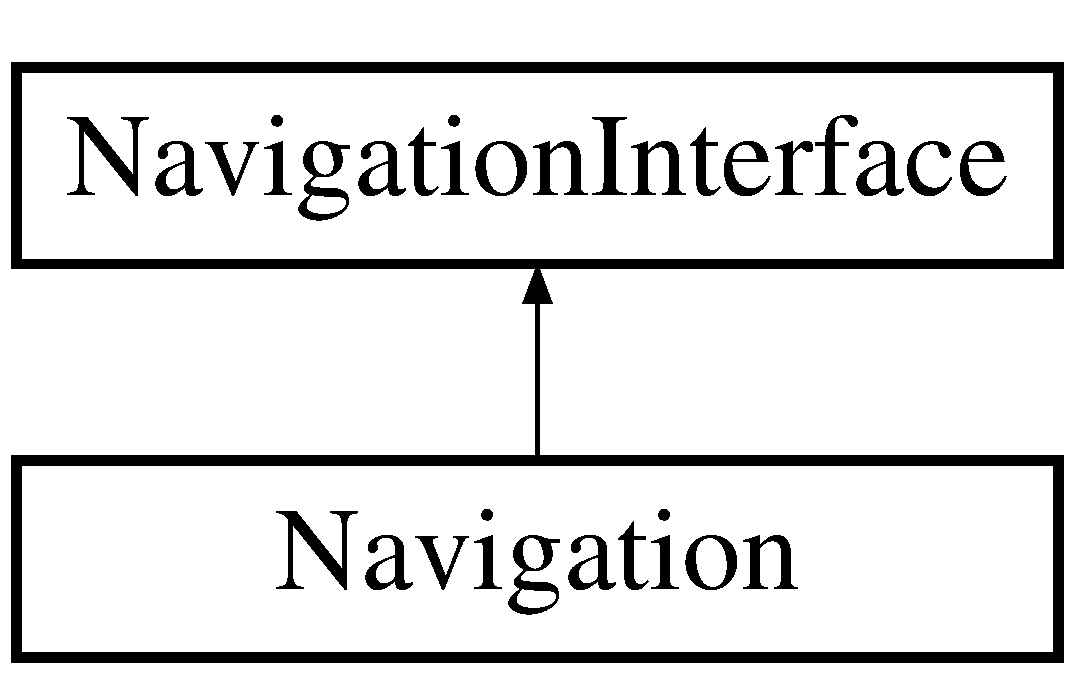
\includegraphics[height=2.000000cm]{classNavigation}
\end{center}
\end{figure}
\subsection*{Public Member Functions}
\begin{DoxyCompactItemize}
\item 
\hyperlink{classNavigation_a81fdffdefe46340da5fa6c570066b42b}{Navigation} ()
\begin{DoxyCompactList}\small\item\em Construct a new \hyperlink{classNavigation}{Navigation} object. \end{DoxyCompactList}\item 
\mbox{\Hypertarget{classNavigation_addd4022d716df48f4e55a1db69361ba7}\label{classNavigation_addd4022d716df48f4e55a1db69361ba7}} 
\hyperlink{classNavigation_addd4022d716df48f4e55a1db69361ba7}{$\sim$\+Navigation} ()
\begin{DoxyCompactList}\small\item\em Destroy the \hyperlink{classNavigation}{Navigation} object. \end{DoxyCompactList}\item 
double \hyperlink{classNavigation_ac417c0408968151493e5dccefae38bc7}{get\+Distance\+From\+Base} (\hyperlink{structPose}{Pose})
\begin{DoxyCompactList}\small\item\em Get the Distance From Base object relative to the base. \end{DoxyCompactList}\item 
void \hyperlink{classNavigation_a91cfc3f3fa511684efd25c7a03a9a7c6}{navigate} (\hyperlink{structPose}{Pose} \&, \hyperlink{structPose}{Pose})
\begin{DoxyCompactList}\small\item\em Wll navigate in the given airspace and set values to verify that the friendly in the airspace. \end{DoxyCompactList}\item 
double \hyperlink{classNavigation_a18d539b159c80fd2d1af2021ad6d3947}{get\+Orientation} (\hyperlink{structPose}{Pose}, \hyperlink{structPose}{Pose})
\begin{DoxyCompactList}\small\item\em Get the Orientation object of the aircraft in space. \end{DoxyCompactList}\item 
double \hyperlink{classNavigation_a9aef484e223556a207734159612fb2c9}{get\+Linear\+Velocity} ()
\begin{DoxyCompactList}\small\item\em Get the Linear Velocity object of aircraft. \end{DoxyCompactList}\item 
double \hyperlink{classNavigation_a412ff177cefb3c4ddaf87daab3fe4c4c}{get\+Angular\+Speed} ()
\begin{DoxyCompactList}\small\item\em Get the Angular Speed object of aircraft. \end{DoxyCompactList}\item 
\hyperlink{structPose}{Pose} \hyperlink{classNavigation_af82fc8cc1546fa2a54e8a8651c1adc80}{get\+Current\+Pose} ()
\begin{DoxyCompactList}\small\item\em Get the Current \hyperlink{structPose}{Pose} object in space. \end{DoxyCompactList}\item 
bool \hyperlink{classNavigation_a4d4d752128c5069db8fcfd969dc22909}{is\+Friendly\+In\+Air\+Space} ()
\begin{DoxyCompactList}\small\item\em will be analysed in friendly aircraft is within the airspace \end{DoxyCompactList}\item 
void \hyperlink{classNavigation_a4f6dcaba60a955746a18760fdb418490}{pure\+Pursuit} (const \hyperlink{structRangeBearingStamped}{Range\+Bearing\+Stamped} \&, \hyperlink{structPose}{Pose})
\begin{DoxyCompactList}\small\item\em The pure pursuit algorithm will compute the angle gama in order to chase the bogies. \end{DoxyCompactList}\end{DoxyCompactItemize}


\subsection{Detailed Description}
The \hyperlink{classNavigation}{Navigation} class will inherit from \hyperlink{classNavigationInterface}{Navigation\+Interface} and will allow to control the friendly and elaborate pure pursuit. 

\subsection{Constructor \& Destructor Documentation}
\mbox{\Hypertarget{classNavigation_a81fdffdefe46340da5fa6c570066b42b}\label{classNavigation_a81fdffdefe46340da5fa6c570066b42b}} 
\index{Navigation@{Navigation}!Navigation@{Navigation}}
\index{Navigation@{Navigation}!Navigation@{Navigation}}
\subsubsection{\texorpdfstring{Navigation()}{Navigation()}}
{\footnotesize\ttfamily Navigation\+::\+Navigation (\begin{DoxyParamCaption}{ }\end{DoxyParamCaption})}



Construct a new \hyperlink{classNavigation}{Navigation} object. 

\begin{DoxyNote}{Note}
Will set angular speed to zero and linear velocity to maximum, Will set to true friendly\+\_\+inside\+\_\+ boolean 
\end{DoxyNote}


\subsection{Member Function Documentation}
\mbox{\Hypertarget{classNavigation_a412ff177cefb3c4ddaf87daab3fe4c4c}\label{classNavigation_a412ff177cefb3c4ddaf87daab3fe4c4c}} 
\index{Navigation@{Navigation}!get\+Angular\+Speed@{get\+Angular\+Speed}}
\index{get\+Angular\+Speed@{get\+Angular\+Speed}!Navigation@{Navigation}}
\subsubsection{\texorpdfstring{get\+Angular\+Speed()}{getAngularSpeed()}}
{\footnotesize\ttfamily double Navigation\+::get\+Angular\+Speed (\begin{DoxyParamCaption}{ }\end{DoxyParamCaption})\hspace{0.3cm}{\ttfamily [virtual]}}



Get the Angular Speed object of aircraft. 

\begin{DoxyReturn}{Returns}
double Angular Speed in rad/s 
\end{DoxyReturn}


Implements \hyperlink{classNavigationInterface_a9fda3919f625414f9fe68dd03deb3130}{Navigation\+Interface}.

\mbox{\Hypertarget{classNavigation_af82fc8cc1546fa2a54e8a8651c1adc80}\label{classNavigation_af82fc8cc1546fa2a54e8a8651c1adc80}} 
\index{Navigation@{Navigation}!get\+Current\+Pose@{get\+Current\+Pose}}
\index{get\+Current\+Pose@{get\+Current\+Pose}!Navigation@{Navigation}}
\subsubsection{\texorpdfstring{get\+Current\+Pose()}{getCurrentPose()}}
{\footnotesize\ttfamily \hyperlink{structPose}{Pose} Navigation\+::get\+Current\+Pose (\begin{DoxyParamCaption}{ }\end{DoxyParamCaption})\hspace{0.3cm}{\ttfamily [virtual]}}



Get the Current \hyperlink{structPose}{Pose} object in space. 

\begin{DoxyReturn}{Returns}
\hyperlink{structPose}{Pose} of aircraft 
\end{DoxyReturn}


Implements \hyperlink{classNavigationInterface_ab37e23f5f838c02d7768d2f02b1fe429}{Navigation\+Interface}.

\mbox{\Hypertarget{classNavigation_ac417c0408968151493e5dccefae38bc7}\label{classNavigation_ac417c0408968151493e5dccefae38bc7}} 
\index{Navigation@{Navigation}!get\+Distance\+From\+Base@{get\+Distance\+From\+Base}}
\index{get\+Distance\+From\+Base@{get\+Distance\+From\+Base}!Navigation@{Navigation}}
\subsubsection{\texorpdfstring{get\+Distance\+From\+Base()}{getDistanceFromBase()}}
{\footnotesize\ttfamily double Navigation\+::get\+Distance\+From\+Base (\begin{DoxyParamCaption}\item[{\hyperlink{structPose}{Pose}}]{Pose }\end{DoxyParamCaption})}



Get the Distance From Base object relative to the base. 


\begin{DoxyParams}[1]{Parameters}
\mbox{\tt in}  & {\em \hyperlink{structPose}{Pose}} & of the airscraft \\
\hline
\end{DoxyParams}
\begin{DoxyReturn}{Returns}
double of tangetial distance 
\end{DoxyReturn}
\mbox{\Hypertarget{classNavigation_a9aef484e223556a207734159612fb2c9}\label{classNavigation_a9aef484e223556a207734159612fb2c9}} 
\index{Navigation@{Navigation}!get\+Linear\+Velocity@{get\+Linear\+Velocity}}
\index{get\+Linear\+Velocity@{get\+Linear\+Velocity}!Navigation@{Navigation}}
\subsubsection{\texorpdfstring{get\+Linear\+Velocity()}{getLinearVelocity()}}
{\footnotesize\ttfamily double Navigation\+::get\+Linear\+Velocity (\begin{DoxyParamCaption}{ }\end{DoxyParamCaption})\hspace{0.3cm}{\ttfamily [virtual]}}



Get the Linear Velocity object of aircraft. 

\begin{DoxyReturn}{Returns}
double Linear Velocity in m/s 
\end{DoxyReturn}


Implements \hyperlink{classNavigationInterface_aa5c9df2654078875f72368e919e28432}{Navigation\+Interface}.

\mbox{\Hypertarget{classNavigation_a18d539b159c80fd2d1af2021ad6d3947}\label{classNavigation_a18d539b159c80fd2d1af2021ad6d3947}} 
\index{Navigation@{Navigation}!get\+Orientation@{get\+Orientation}}
\index{get\+Orientation@{get\+Orientation}!Navigation@{Navigation}}
\subsubsection{\texorpdfstring{get\+Orientation()}{getOrientation()}}
{\footnotesize\ttfamily double Navigation\+::get\+Orientation (\begin{DoxyParamCaption}\item[{\hyperlink{structPose}{Pose}}]{Pose\+\_\+reference,  }\item[{\hyperlink{structPose}{Pose}}]{Pose }\end{DoxyParamCaption})}



Get the Orientation object of the aircraft in space. 


\begin{DoxyParams}[1]{Parameters}
\mbox{\tt in}  & {\em \hyperlink{structPose}{Pose}} & reference pose \\
\hline
\mbox{\tt in}  & {\em \hyperlink{structPose}{Pose}} & actual given pose \\
\hline
\end{DoxyParams}
\begin{DoxyReturn}{Returns}
double of orientation 
\end{DoxyReturn}
\mbox{\Hypertarget{classNavigation_a4d4d752128c5069db8fcfd969dc22909}\label{classNavigation_a4d4d752128c5069db8fcfd969dc22909}} 
\index{Navigation@{Navigation}!is\+Friendly\+In\+Air\+Space@{is\+Friendly\+In\+Air\+Space}}
\index{is\+Friendly\+In\+Air\+Space@{is\+Friendly\+In\+Air\+Space}!Navigation@{Navigation}}
\subsubsection{\texorpdfstring{is\+Friendly\+In\+Air\+Space()}{isFriendlyInAirSpace()}}
{\footnotesize\ttfamily bool Navigation\+::is\+Friendly\+In\+Air\+Space (\begin{DoxyParamCaption}{ }\end{DoxyParamCaption})}



will be analysed in friendly aircraft is within the airspace 

\begin{DoxyReturn}{Returns}
true friendly aircraft is inside the airspace 

false friendly aircraft is not inside the airspace 
\end{DoxyReturn}
\mbox{\Hypertarget{classNavigation_a91cfc3f3fa511684efd25c7a03a9a7c6}\label{classNavigation_a91cfc3f3fa511684efd25c7a03a9a7c6}} 
\index{Navigation@{Navigation}!navigate@{navigate}}
\index{navigate@{navigate}!Navigation@{Navigation}}
\subsubsection{\texorpdfstring{navigate()}{navigate()}}
{\footnotesize\ttfamily void Navigation\+::navigate (\begin{DoxyParamCaption}\item[{\hyperlink{structPose}{Pose} \&}]{friendly\+\_\+simulator,  }\item[{\hyperlink{structPose}{Pose}}]{friendly }\end{DoxyParamCaption})}



Wll navigate in the given airspace and set values to verify that the friendly in the airspace. 

\begin{DoxyNote}{Note}
Will Consider a threshold angle and the position in space with a given buffer in order to steer the aircraft and avoid leaving the airspace Will keep track of bolean of friendly\+\_\+inside\+\_\+ 
\end{DoxyNote}

\begin{DoxyParams}[1]{Parameters}
\mbox{\tt in}  & {\em \hyperlink{structPose}{Pose}} & pass a reference pose for analysis \\
\hline
\mbox{\tt in}  & {\em \hyperlink{structPose}{Pose}} & actual pose of the aircraft \\
\hline
\end{DoxyParams}
\mbox{\Hypertarget{classNavigation_a4f6dcaba60a955746a18760fdb418490}\label{classNavigation_a4f6dcaba60a955746a18760fdb418490}} 
\index{Navigation@{Navigation}!pure\+Pursuit@{pure\+Pursuit}}
\index{pure\+Pursuit@{pure\+Pursuit}!Navigation@{Navigation}}
\subsubsection{\texorpdfstring{pure\+Pursuit()}{purePursuit()}}
{\footnotesize\ttfamily void Navigation\+::pure\+Pursuit (\begin{DoxyParamCaption}\item[{const \hyperlink{structRangeBearingStamped}{Range\+Bearing\+Stamped} \&}]{bogie\+\_\+target,  }\item[{\hyperlink{structPose}{Pose}}]{friendly }\end{DoxyParamCaption})}



The pure pursuit algorithm will compute the angle gama in order to chase the bogies. 

\begin{DoxyNote}{Note}
This also implements a PI controller to facilitate the steering of the friendly 
\end{DoxyNote}

\begin{DoxyParams}[1]{Parameters}
\mbox{\tt in}  & {\em \hyperlink{structRangeBearingStamped}{Range\+Bearing\+Stamped}} & in order track the angle of the bogie \\
\hline
\mbox{\tt in}  & {\em \hyperlink{structPose}{Pose}} & in order to track the position of the friendly as the new reference \\
\hline
\end{DoxyParams}


The documentation for this class was generated from the following files\+:\begin{DoxyCompactItemize}
\item 
/home/esteban/git/pfms-\/2020a-\/esteban-\/andrade/scratch/\+Assignment3/\+Submission/a3/\hyperlink{Navigation_8h}{Navigation.\+h}\item 
/home/esteban/git/pfms-\/2020a-\/esteban-\/andrade/scratch/\+Assignment3/\+Submission/a3/Navigation.\+cpp\end{DoxyCompactItemize}

\hypertarget{classNavigationInterface}{}\section{Navigation\+Interface Class Reference}
\label{classNavigationInterface}\index{Navigation\+Interface@{Navigation\+Interface}}


The \hyperlink{classNavigationInterface}{Navigation\+Interface} class will aid to create subsequent navigation child classes.  




{\ttfamily \#include $<$Navigation\+Interface.\+h$>$}

Inheritance diagram for Navigation\+Interface\+:\begin{figure}[H]
\begin{center}
\leavevmode
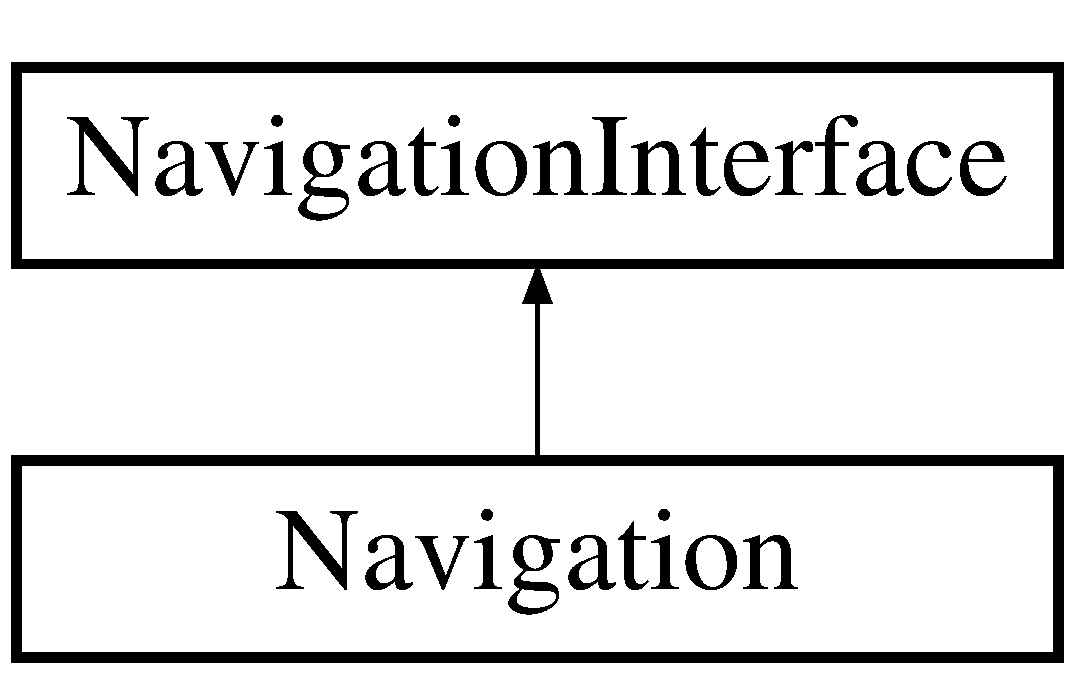
\includegraphics[height=2.000000cm]{classNavigationInterface}
\end{center}
\end{figure}
\subsection*{Public Member Functions}
\begin{DoxyCompactItemize}
\item 
\mbox{\Hypertarget{classNavigationInterface_ae33d4f7b177fb85615bba6d144a5cb6b}\label{classNavigationInterface_ae33d4f7b177fb85615bba6d144a5cb6b}} 
\hyperlink{classNavigationInterface_ae33d4f7b177fb85615bba6d144a5cb6b}{Navigation\+Interface} ()
\begin{DoxyCompactList}\small\item\em Construct a new \hyperlink{classNavigation}{Navigation} Interface object of abstract class. \end{DoxyCompactList}\item 
\mbox{\Hypertarget{classNavigationInterface_a1f3b72da52b5f8692303f9dcae118f05}\label{classNavigationInterface_a1f3b72da52b5f8692303f9dcae118f05}} 
\hyperlink{classNavigationInterface_a1f3b72da52b5f8692303f9dcae118f05}{$\sim$\+Navigation\+Interface} ()
\begin{DoxyCompactList}\small\item\em Destroy the \hyperlink{classNavigation}{Navigation} Interface object of abstract class. \end{DoxyCompactList}\item 
virtual double \hyperlink{classNavigationInterface_a9fda3919f625414f9fe68dd03deb3130}{get\+Angular\+Speed} ()=0
\begin{DoxyCompactList}\small\item\em Get the Angular Speed object in rad/s. \end{DoxyCompactList}\item 
virtual double \hyperlink{classNavigationInterface_aa5c9df2654078875f72368e919e28432}{get\+Linear\+Velocity} ()=0
\begin{DoxyCompactList}\small\item\em Get the Linear Velocity object in m/s. \end{DoxyCompactList}\item 
virtual \hyperlink{structPose}{Pose} \hyperlink{classNavigationInterface_ab37e23f5f838c02d7768d2f02b1fe429}{get\+Current\+Pose} ()=0
\begin{DoxyCompactList}\small\item\em Get the Current \hyperlink{structPose}{Pose} object the pose object in space. \end{DoxyCompactList}\end{DoxyCompactItemize}


\subsection{Detailed Description}
The \hyperlink{classNavigationInterface}{Navigation\+Interface} class will aid to create subsequent navigation child classes. 

\subsection{Member Function Documentation}
\mbox{\Hypertarget{classNavigationInterface_a9fda3919f625414f9fe68dd03deb3130}\label{classNavigationInterface_a9fda3919f625414f9fe68dd03deb3130}} 
\index{Navigation\+Interface@{Navigation\+Interface}!get\+Angular\+Speed@{get\+Angular\+Speed}}
\index{get\+Angular\+Speed@{get\+Angular\+Speed}!Navigation\+Interface@{Navigation\+Interface}}
\subsubsection{\texorpdfstring{get\+Angular\+Speed()}{getAngularSpeed()}}
{\footnotesize\ttfamily virtual double Navigation\+Interface\+::get\+Angular\+Speed (\begin{DoxyParamCaption}{ }\end{DoxyParamCaption})\hspace{0.3cm}{\ttfamily [pure virtual]}}



Get the Angular Speed object in rad/s. 

\begin{DoxyReturn}{Returns}
double of Angular Speed 
\end{DoxyReturn}


Implemented in \hyperlink{classNavigation_a412ff177cefb3c4ddaf87daab3fe4c4c}{Navigation}.

\mbox{\Hypertarget{classNavigationInterface_ab37e23f5f838c02d7768d2f02b1fe429}\label{classNavigationInterface_ab37e23f5f838c02d7768d2f02b1fe429}} 
\index{Navigation\+Interface@{Navigation\+Interface}!get\+Current\+Pose@{get\+Current\+Pose}}
\index{get\+Current\+Pose@{get\+Current\+Pose}!Navigation\+Interface@{Navigation\+Interface}}
\subsubsection{\texorpdfstring{get\+Current\+Pose()}{getCurrentPose()}}
{\footnotesize\ttfamily virtual \hyperlink{structPose}{Pose} Navigation\+Interface\+::get\+Current\+Pose (\begin{DoxyParamCaption}{ }\end{DoxyParamCaption})\hspace{0.3cm}{\ttfamily [pure virtual]}}



Get the Current \hyperlink{structPose}{Pose} object the pose object in space. 

\begin{DoxyReturn}{Returns}
\hyperlink{structPose}{Pose} of position and orientation 
\end{DoxyReturn}


Implemented in \hyperlink{classNavigation_af82fc8cc1546fa2a54e8a8651c1adc80}{Navigation}.

\mbox{\Hypertarget{classNavigationInterface_aa5c9df2654078875f72368e919e28432}\label{classNavigationInterface_aa5c9df2654078875f72368e919e28432}} 
\index{Navigation\+Interface@{Navigation\+Interface}!get\+Linear\+Velocity@{get\+Linear\+Velocity}}
\index{get\+Linear\+Velocity@{get\+Linear\+Velocity}!Navigation\+Interface@{Navigation\+Interface}}
\subsubsection{\texorpdfstring{get\+Linear\+Velocity()}{getLinearVelocity()}}
{\footnotesize\ttfamily virtual double Navigation\+Interface\+::get\+Linear\+Velocity (\begin{DoxyParamCaption}{ }\end{DoxyParamCaption})\hspace{0.3cm}{\ttfamily [pure virtual]}}



Get the Linear Velocity object in m/s. 

\begin{DoxyReturn}{Returns}
double of Linear Velocity 
\end{DoxyReturn}


Implemented in \hyperlink{classNavigation_a9aef484e223556a207734159612fb2c9}{Navigation}.



The documentation for this class was generated from the following file\+:\begin{DoxyCompactItemize}
\item 
/home/esteban/git/pfms-\/2020a-\/esteban-\/andrade/scratch/\+Assignment3/a3/\hyperlink{NavigationInterface_8h}{Navigation\+Interface.\+h}\end{DoxyCompactItemize}

\hypertarget{structPose}{}\section{Pose Struct Reference}
\label{structPose}\index{Pose@{Pose}}
\subsection*{Public Attributes}
\begin{DoxyCompactItemize}
\item 
\hyperlink{structGlobalOrd}{Global\+Ord} \hyperlink{structPose_aba2eb8f799d1d392757d6c9490179720}{position}
\item 
double \hyperlink{structPose_a94d058eaab99263c6ab43bf53f4ebd9a}{orientation}
\end{DoxyCompactItemize}


\subsection{Member Data Documentation}
\mbox{\Hypertarget{structPose_a94d058eaab99263c6ab43bf53f4ebd9a}\label{structPose_a94d058eaab99263c6ab43bf53f4ebd9a}} 
\index{Pose@{Pose}!orientation@{orientation}}
\index{orientation@{orientation}!Pose@{Pose}}
\subsubsection{\texorpdfstring{orientation}{orientation}}
{\footnotesize\ttfamily double Pose\+::orientation}

Orientation (radians) \mbox{\Hypertarget{structPose_aba2eb8f799d1d392757d6c9490179720}\label{structPose_aba2eb8f799d1d392757d6c9490179720}} 
\index{Pose@{Pose}!position@{position}}
\index{position@{position}!Pose@{Pose}}
\subsubsection{\texorpdfstring{position}{position}}
{\footnotesize\ttfamily \hyperlink{structGlobalOrd}{Global\+Ord} Pose\+::position}

Global position (metres) 

The documentation for this struct was generated from the following file\+:\begin{DoxyCompactItemize}
\item 
/home/esteban/git/pfms-\/2020a-\/esteban-\/andrade/scratch/\+Assignment3/\+Submission/a3/dep/bionic/\hyperlink{bionic_2types_8h}{types.\+h}\end{DoxyCompactItemize}

\hypertarget{structRangeBearingStamped}{}\section{Range\+Bearing\+Stamped Struct Reference}
\label{structRangeBearingStamped}\index{Range\+Bearing\+Stamped@{Range\+Bearing\+Stamped}}
\subsection*{Public Attributes}
\begin{DoxyCompactItemize}
\item 
double \hyperlink{structRangeBearingStamped_af49767ebfdc4e481cab3ec2453f83884}{range}
\item 
double \hyperlink{structRangeBearingStamped_a7fffdf2e1776060acadc87083740a1da}{bearing}
\item 
long \hyperlink{structRangeBearingStamped_a7803974f4f1e9de3469b21dae3289530}{timestamp}
\end{DoxyCompactItemize}


\subsection{Member Data Documentation}
\mbox{\Hypertarget{structRangeBearingStamped_a7fffdf2e1776060acadc87083740a1da}\label{structRangeBearingStamped_a7fffdf2e1776060acadc87083740a1da}} 
\index{Range\+Bearing\+Stamped@{Range\+Bearing\+Stamped}!bearing@{bearing}}
\index{bearing@{bearing}!Range\+Bearing\+Stamped@{Range\+Bearing\+Stamped}}
\subsubsection{\texorpdfstring{bearing}{bearing}}
{\footnotesize\ttfamily double Range\+Bearing\+Stamped\+::bearing}

The bearing (bearing reading) in radians \mbox{\Hypertarget{structRangeBearingStamped_af49767ebfdc4e481cab3ec2453f83884}\label{structRangeBearingStamped_af49767ebfdc4e481cab3ec2453f83884}} 
\index{Range\+Bearing\+Stamped@{Range\+Bearing\+Stamped}!range@{range}}
\index{range@{range}!Range\+Bearing\+Stamped@{Range\+Bearing\+Stamped}}
\subsubsection{\texorpdfstring{range}{range}}
{\footnotesize\ttfamily double Range\+Bearing\+Stamped\+::range}

$<$ Contains a timestamped range/bearing reading The range (distance reading) in metres \mbox{\Hypertarget{structRangeBearingStamped_a7803974f4f1e9de3469b21dae3289530}\label{structRangeBearingStamped_a7803974f4f1e9de3469b21dae3289530}} 
\index{Range\+Bearing\+Stamped@{Range\+Bearing\+Stamped}!timestamp@{timestamp}}
\index{timestamp@{timestamp}!Range\+Bearing\+Stamped@{Range\+Bearing\+Stamped}}
\subsubsection{\texorpdfstring{timestamp}{timestamp}}
{\footnotesize\ttfamily long Range\+Bearing\+Stamped\+::timestamp}

Timestamp (milliseconds) 

The documentation for this struct was generated from the following file\+:\begin{DoxyCompactItemize}
\item 
/home/esteban/git/pfms-\/2020a-\/esteban-\/andrade/scratch/\+Assignment3/a3/dep/bionic/\hyperlink{bionic_2types_8h}{types.\+h}\end{DoxyCompactItemize}

\hypertarget{structRangeVelocityStamped}{}\section{Range\+Velocity\+Stamped Struct Reference}
\label{structRangeVelocityStamped}\index{Range\+Velocity\+Stamped@{Range\+Velocity\+Stamped}}
\subsection*{Public Attributes}
\begin{DoxyCompactItemize}
\item 
double \hyperlink{structRangeVelocityStamped_ae635d3c25ade1a2f5c52f62442eb0bf9}{range}
\item 
double \hyperlink{structRangeVelocityStamped_a17777401a22b59317e92666f03f7fc88}{velocity}
\item 
long \hyperlink{structRangeVelocityStamped_a3fec5547c45ed9c80e69ff7e38d9ef99}{timestamp}
\end{DoxyCompactItemize}


\subsection{Member Data Documentation}
\mbox{\Hypertarget{structRangeVelocityStamped_ae635d3c25ade1a2f5c52f62442eb0bf9}\label{structRangeVelocityStamped_ae635d3c25ade1a2f5c52f62442eb0bf9}} 
\index{Range\+Velocity\+Stamped@{Range\+Velocity\+Stamped}!range@{range}}
\index{range@{range}!Range\+Velocity\+Stamped@{Range\+Velocity\+Stamped}}
\subsubsection{\texorpdfstring{range}{range}}
{\footnotesize\ttfamily double Range\+Velocity\+Stamped\+::range}

$<$ Contains a timestamped range/bearing reading The range (distance reading) in metres \mbox{\Hypertarget{structRangeVelocityStamped_a3fec5547c45ed9c80e69ff7e38d9ef99}\label{structRangeVelocityStamped_a3fec5547c45ed9c80e69ff7e38d9ef99}} 
\index{Range\+Velocity\+Stamped@{Range\+Velocity\+Stamped}!timestamp@{timestamp}}
\index{timestamp@{timestamp}!Range\+Velocity\+Stamped@{Range\+Velocity\+Stamped}}
\subsubsection{\texorpdfstring{timestamp}{timestamp}}
{\footnotesize\ttfamily long Range\+Velocity\+Stamped\+::timestamp}

Timestamp (milliseconds) \mbox{\Hypertarget{structRangeVelocityStamped_a17777401a22b59317e92666f03f7fc88}\label{structRangeVelocityStamped_a17777401a22b59317e92666f03f7fc88}} 
\index{Range\+Velocity\+Stamped@{Range\+Velocity\+Stamped}!velocity@{velocity}}
\index{velocity@{velocity}!Range\+Velocity\+Stamped@{Range\+Velocity\+Stamped}}
\subsubsection{\texorpdfstring{velocity}{velocity}}
{\footnotesize\ttfamily double Range\+Velocity\+Stamped\+::velocity}

Linear velocity (metres/second) 

The documentation for this struct was generated from the following file\+:\begin{DoxyCompactItemize}
\item 
/home/esteban/git/pfms-\/2020a-\/esteban-\/andrade/scratch/\+Assignment3/a3/dep/bionic/\hyperlink{bionic_2types_8h}{types.\+h}\end{DoxyCompactItemize}

\hypertarget{classScanner}{}\section{Scanner Class Reference}
\label{classScanner}\index{Scanner@{Scanner}}


The class \hyperlink{classScanner}{Scanner} will perform all the analysis relative to the aircraft and base in respect to the bogies.  




{\ttfamily \#include $<$Scanner.\+h$>$}

Inheritance diagram for Scanner\+:\begin{figure}[H]
\begin{center}
\leavevmode
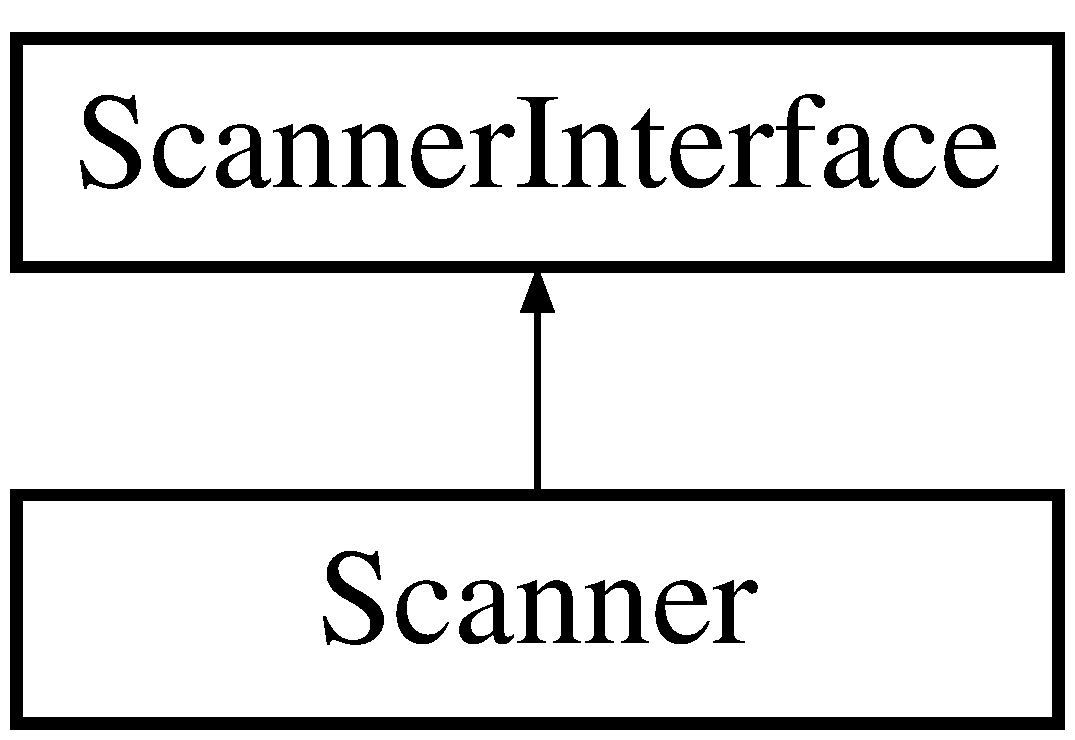
\includegraphics[height=2.000000cm]{classScanner}
\end{center}
\end{figure}
\subsection*{Public Member Functions}
\begin{DoxyCompactItemize}
\item 
\mbox{\Hypertarget{classScanner_acc995a4b67a10d2652ce00afed14f497}\label{classScanner_acc995a4b67a10d2652ce00afed14f497}} 
\hyperlink{classScanner_acc995a4b67a10d2652ce00afed14f497}{Scanner} ()
\begin{DoxyCompactList}\small\item\em Construct a new \hyperlink{classScanner}{Scanner} object. \end{DoxyCompactList}\item 
\mbox{\Hypertarget{classScanner_a39f85e20f3ca942fd0a8e4bce88c27c7}\label{classScanner_a39f85e20f3ca942fd0a8e4bce88c27c7}} 
\hyperlink{classScanner_a39f85e20f3ca942fd0a8e4bce88c27c7}{$\sim$\+Scanner} ()
\begin{DoxyCompactList}\small\item\em Destroy the \hyperlink{classScanner}{Scanner} object. \end{DoxyCompactList}\item 
void \hyperlink{classScanner_a846ec9883243c9837e0a910cd82e969d}{determine\+Target} (\hyperlink{structPose}{Pose}, std\+::vector$<$ \hyperlink{structRangeBearingStamped}{Range\+Bearing\+Stamped} $>$)
\begin{DoxyCompactList}\small\item\em Will determine the target bogie. it will select the most appropiate bogie and store its position in x and y. \end{DoxyCompactList}\item 
void \hyperlink{classScanner_ad0f7c663c60e8315c5f99935de8e9ecb}{friendly\+Relative\+Base} (\hyperlink{structPose}{Pose} \&)
\begin{DoxyCompactList}\small\item\em Will get and analise the distance from the base relative to the friendly. \end{DoxyCompactList}\item 
void \hyperlink{classScanner_ad18851f19a61b642c699f425b62911a4}{base\+Scan} (std\+::vector$<$ \hyperlink{structRangeVelocityStamped}{Range\+Velocity\+Stamped} $>$ \&)
\begin{DoxyCompactList}\small\item\em Will Scan and store the Values from the friendly scanner. \end{DoxyCompactList}\item 
void \hyperlink{classScanner_a61dd33aeecd220e4dec5f9cbd6403f9e}{air\+Craft\+Scan} (std\+::vector$<$ \hyperlink{structRangeBearingStamped}{Range\+Bearing\+Stamped} $>$ \&)
\begin{DoxyCompactList}\small\item\em Will analyse and the passed vector of \hyperlink{structRangeVelocityStamped}{Range\+Velocity\+Stamped} and it will sort the results. \end{DoxyCompactList}\item 
std\+::vector$<$ \hyperlink{structRangeVelocityStamped}{Range\+Velocity\+Stamped} $>$ \hyperlink{classScanner_a59590dd900ab1c5cc362fa4a00df533d}{get\+Base\+Scan\+Results} ()
\begin{DoxyCompactList}\small\item\em Get the Base Scan Results object from base scam. \end{DoxyCompactList}\item 
std\+::vector$<$ \hyperlink{structRangeBearingStamped}{Range\+Bearing\+Stamped} $>$ \hyperlink{classScanner_a27b2ba73647d40946e00bceb824712e9}{get\+Friendly\+Scan\+Results} ()
\begin{DoxyCompactList}\small\item\em Get the Friendly Scan Results object from aircraft scan. \end{DoxyCompactList}\item 
std\+::vector$<$ std\+::pair$<$ double, double $>$ $>$ \hyperlink{classScanner_a556ac0598666bf9543099daef4655d6b}{get\+Target} ()
\begin{DoxyCompactList}\small\item\em Get the Target object of the bogie. \end{DoxyCompactList}\item 
\mbox{\Hypertarget{classScanner_a95dea82a0db3f7ca8cf5152c85f89239}\label{classScanner_a95dea82a0db3f7ca8cf5152c85f89239}} 
void \hyperlink{classScanner_a95dea82a0db3f7ca8cf5152c85f89239}{reset\+Data} ()
\begin{DoxyCompactList}\small\item\em Will reset all the data and S\+TL containers. \end{DoxyCompactList}\item 
std\+::vector$<$ std\+::pair$<$ double, double $>$ $>$ \hyperlink{classScanner_a26f1e15d585005c467740b4bed4329c0}{get\+Base\+Scan} ()
\begin{DoxyCompactList}\small\item\em Get the Base Scan object from the base Scan. \end{DoxyCompactList}\item 
std\+::vector$<$ std\+::pair$<$ double, double $>$ $>$ \hyperlink{classScanner_a32f7e7f5ff6ac8f048263e26b059aae9}{get\+Friendly\+Scan} ()
\begin{DoxyCompactList}\small\item\em Get the Friendly Scan object from the \hyperlink{structAircraft}{Aircraft} scan. \end{DoxyCompactList}\item 
std\+::vector$<$ std\+::pair$<$ double, double $>$ $>$ \hyperlink{classScanner_a5b8ec13e023aef168abc91716d22bbb2}{get\+Base\+To\+Friendly} ()
\begin{DoxyCompactList}\small\item\em Get the Base To Friendly object relative to the base. \end{DoxyCompactList}\item 
int \hyperlink{classScanner_a22fe48ec9b56a6475f5e8a8745adca1f}{get\+Bogie\+Index} ()
\begin{DoxyCompactList}\small\item\em Get the Bogie Index object. \end{DoxyCompactList}\item 
void \hyperlink{classScanner_ae744985c5a046805010a9388cedaa006}{predict\+Target} (std\+::vector$<$ \hyperlink{structRangeBearingStamped}{Range\+Bearing\+Stamped} $>$ \&, std\+::vector$<$ \hyperlink{structRangeBearingStamped}{Range\+Bearing\+Stamped} $>$ \&)
\begin{DoxyCompactList}\small\item\em will Analyse the predicted position and compute the velocity vector \end{DoxyCompactList}\item 
std\+::vector$<$ double $>$ \hyperlink{classScanner_ac9b03f1f8b6f38f6f8144affa6be9854}{get\+Object\+Velocity} ()
\begin{DoxyCompactList}\small\item\em Get the Object Velocity object in Scalar. \end{DoxyCompactList}\item 
std\+::vector$<$ std\+::pair$<$ double, double $>$ $>$ \hyperlink{classScanner_a4f9ba72b2339cad7e3cb7ffe46196ea2}{get\+Predicted\+Target} ()
\begin{DoxyCompactList}\small\item\em Get the Predicted Target object in position x and y. \end{DoxyCompactList}\item 
double \hyperlink{classScanner_a222da6748f943d345a926d5a7094795e}{get\+Bearing\+Angle} ()
\begin{DoxyCompactList}\small\item\em Get the Bearing Angle object relative to the friendly and bogie. \end{DoxyCompactList}\item 
std\+::vector$<$ std\+::pair$<$ double, double $>$ $>$ \hyperlink{classScanner_aa551cad3b1137f4fbe052181f09f987f}{get\+Velocity\+Vector} ()
\begin{DoxyCompactList}\small\item\em Get the Velocity Vector object. \end{DoxyCompactList}\item 
double \hyperlink{classScanner_a3ba854fbf61ce01180479f2d9fbf11f9}{get\+Orientation\+Prediction} ()
\begin{DoxyCompactList}\small\item\em Get the Orientation Prediction object of the bogie. \end{DoxyCompactList}\end{DoxyCompactItemize}


\subsection{Detailed Description}
The class \hyperlink{classScanner}{Scanner} will perform all the analysis relative to the aircraft and base in respect to the bogies. 

\subsection{Member Function Documentation}
\mbox{\Hypertarget{classScanner_a61dd33aeecd220e4dec5f9cbd6403f9e}\label{classScanner_a61dd33aeecd220e4dec5f9cbd6403f9e}} 
\index{Scanner@{Scanner}!air\+Craft\+Scan@{air\+Craft\+Scan}}
\index{air\+Craft\+Scan@{air\+Craft\+Scan}!Scanner@{Scanner}}
\subsubsection{\texorpdfstring{air\+Craft\+Scan()}{airCraftScan()}}
{\footnotesize\ttfamily void Scanner\+::air\+Craft\+Scan (\begin{DoxyParamCaption}\item[{std\+::vector$<$ \hyperlink{structRangeBearingStamped}{Range\+Bearing\+Stamped} $>$ \&}]{raw\+\_\+scan\+\_\+sim }\end{DoxyParamCaption})}



Will analyse and the passed vector of \hyperlink{structRangeVelocityStamped}{Range\+Velocity\+Stamped} and it will sort the results. 

\begin{DoxyNote}{Note}
Will store the in pairs of range and theta of the bogies relative to the friendly 
\end{DoxyNote}

\begin{DoxyParams}[1]{Parameters}
\mbox{\tt in}  & {\em vector} & \hyperlink{structRangeBearingStamped}{Range\+Bearing\+Stamped} \\
\hline
\end{DoxyParams}
\mbox{\Hypertarget{classScanner_ad18851f19a61b642c699f425b62911a4}\label{classScanner_ad18851f19a61b642c699f425b62911a4}} 
\index{Scanner@{Scanner}!base\+Scan@{base\+Scan}}
\index{base\+Scan@{base\+Scan}!Scanner@{Scanner}}
\subsubsection{\texorpdfstring{base\+Scan()}{baseScan()}}
{\footnotesize\ttfamily void Scanner\+::base\+Scan (\begin{DoxyParamCaption}\item[{std\+::vector$<$ \hyperlink{structRangeVelocityStamped}{Range\+Velocity\+Stamped} $>$ \&}]{base\+\_\+scan\+\_\+sim }\end{DoxyParamCaption})}



Will Scan and store the Values from the friendly scanner. 

\begin{DoxyNote}{Note}
it will Store the range of the scan 
\end{DoxyNote}

\begin{DoxyParams}[1]{Parameters}
\mbox{\tt in}  & {\em Vector} & of \hyperlink{structRangeVelocityStamped}{Range\+Velocity\+Stamped} \\
\hline
\end{DoxyParams}
\mbox{\Hypertarget{classScanner_a846ec9883243c9837e0a910cd82e969d}\label{classScanner_a846ec9883243c9837e0a910cd82e969d}} 
\index{Scanner@{Scanner}!determine\+Target@{determine\+Target}}
\index{determine\+Target@{determine\+Target}!Scanner@{Scanner}}
\subsubsection{\texorpdfstring{determine\+Target()}{determineTarget()}}
{\footnotesize\ttfamily void Scanner\+::determine\+Target (\begin{DoxyParamCaption}\item[{\hyperlink{structPose}{Pose}}]{pose\+\_\+sim,  }\item[{std\+::vector$<$ \hyperlink{structRangeBearingStamped}{Range\+Bearing\+Stamped} $>$}]{friendly\+\_\+scan }\end{DoxyParamCaption})}



Will determine the target bogie. it will select the most appropiate bogie and store its position in x and y. 


\begin{DoxyParams}[1]{Parameters}
\mbox{\tt in}  & {\em \hyperlink{structPose}{Pose}} & of the corresponding bogie object \\
\hline
\mbox{\tt in}  & {\em Vector} & of \hyperlink{structRangeBearingStamped}{Range\+Bearing\+Stamped} in order to analyse the the angle and position \\
\hline
\end{DoxyParams}
\mbox{\Hypertarget{classScanner_ad0f7c663c60e8315c5f99935de8e9ecb}\label{classScanner_ad0f7c663c60e8315c5f99935de8e9ecb}} 
\index{Scanner@{Scanner}!friendly\+Relative\+Base@{friendly\+Relative\+Base}}
\index{friendly\+Relative\+Base@{friendly\+Relative\+Base}!Scanner@{Scanner}}
\subsubsection{\texorpdfstring{friendly\+Relative\+Base()}{friendlyRelativeBase()}}
{\footnotesize\ttfamily void Scanner\+::friendly\+Relative\+Base (\begin{DoxyParamCaption}\item[{\hyperlink{structPose}{Pose} \&}]{friendly\+\_\+to\+\_\+base }\end{DoxyParamCaption})}



Will get and analise the distance from the base relative to the friendly. 

\begin{DoxyNote}{Note}
Will convert the coordinates to tangential distande 
\end{DoxyNote}

\begin{DoxyParams}[1]{Parameters}
\mbox{\tt in}  & {\em \hyperlink{structPose}{Pose}} & of the friendly \\
\hline
\end{DoxyParams}
\mbox{\Hypertarget{classScanner_a26f1e15d585005c467740b4bed4329c0}\label{classScanner_a26f1e15d585005c467740b4bed4329c0}} 
\index{Scanner@{Scanner}!get\+Base\+Scan@{get\+Base\+Scan}}
\index{get\+Base\+Scan@{get\+Base\+Scan}!Scanner@{Scanner}}
\subsubsection{\texorpdfstring{get\+Base\+Scan()}{getBaseScan()}}
{\footnotesize\ttfamily std\+::vector$<$ std\+::pair$<$ double, double $>$ $>$ Scanner\+::get\+Base\+Scan (\begin{DoxyParamCaption}{ }\end{DoxyParamCaption})}



Get the Base Scan object from the base Scan. 

\begin{DoxyNote}{Note}
will return range and time stamp 
\end{DoxyNote}
\begin{DoxyReturn}{Returns}
std\+::vector$<$std\+::pair$<$double, double$>$$>$ Base\+Scan\+Coordinates 
\end{DoxyReturn}
\mbox{\Hypertarget{classScanner_a59590dd900ab1c5cc362fa4a00df533d}\label{classScanner_a59590dd900ab1c5cc362fa4a00df533d}} 
\index{Scanner@{Scanner}!get\+Base\+Scan\+Results@{get\+Base\+Scan\+Results}}
\index{get\+Base\+Scan\+Results@{get\+Base\+Scan\+Results}!Scanner@{Scanner}}
\subsubsection{\texorpdfstring{get\+Base\+Scan\+Results()}{getBaseScanResults()}}
{\footnotesize\ttfamily std\+::vector$<$ \hyperlink{structRangeVelocityStamped}{Range\+Velocity\+Stamped} $>$ Scanner\+::get\+Base\+Scan\+Results (\begin{DoxyParamCaption}{ }\end{DoxyParamCaption})}



Get the Base Scan Results object from base scam. 

\begin{DoxyReturn}{Returns}
std\+::vector$<$\+Range\+Velocity\+Stamped$>$ of Base\+Scan 
\end{DoxyReturn}
\mbox{\Hypertarget{classScanner_a5b8ec13e023aef168abc91716d22bbb2}\label{classScanner_a5b8ec13e023aef168abc91716d22bbb2}} 
\index{Scanner@{Scanner}!get\+Base\+To\+Friendly@{get\+Base\+To\+Friendly}}
\index{get\+Base\+To\+Friendly@{get\+Base\+To\+Friendly}!Scanner@{Scanner}}
\subsubsection{\texorpdfstring{get\+Base\+To\+Friendly()}{getBaseToFriendly()}}
{\footnotesize\ttfamily std\+::vector$<$ std\+::pair$<$ double, double $>$ $>$ Scanner\+::get\+Base\+To\+Friendly (\begin{DoxyParamCaption}{ }\end{DoxyParamCaption})}



Get the Base To Friendly object relative to the base. 

\begin{DoxyNote}{Note}
Will get values of distance and angle 
\end{DoxyNote}
\begin{DoxyReturn}{Returns}
std\+::vector$<$std\+::pair$<$double, double$>$$>$ Base\+To\+Friendly\+Coordinates 
\end{DoxyReturn}
\mbox{\Hypertarget{classScanner_a222da6748f943d345a926d5a7094795e}\label{classScanner_a222da6748f943d345a926d5a7094795e}} 
\index{Scanner@{Scanner}!get\+Bearing\+Angle@{get\+Bearing\+Angle}}
\index{get\+Bearing\+Angle@{get\+Bearing\+Angle}!Scanner@{Scanner}}
\subsubsection{\texorpdfstring{get\+Bearing\+Angle()}{getBearingAngle()}}
{\footnotesize\ttfamily double Scanner\+::get\+Bearing\+Angle (\begin{DoxyParamCaption}{ }\end{DoxyParamCaption})}



Get the Bearing Angle object relative to the friendly and bogie. 

\begin{DoxyReturn}{Returns}
double of bearing angle 
\end{DoxyReturn}
\mbox{\Hypertarget{classScanner_a22fe48ec9b56a6475f5e8a8745adca1f}\label{classScanner_a22fe48ec9b56a6475f5e8a8745adca1f}} 
\index{Scanner@{Scanner}!get\+Bogie\+Index@{get\+Bogie\+Index}}
\index{get\+Bogie\+Index@{get\+Bogie\+Index}!Scanner@{Scanner}}
\subsubsection{\texorpdfstring{get\+Bogie\+Index()}{getBogieIndex()}}
{\footnotesize\ttfamily int Scanner\+::get\+Bogie\+Index (\begin{DoxyParamCaption}{ }\end{DoxyParamCaption})}



Get the Bogie Index object. 

\begin{DoxyReturn}{Returns}
int of bogie index target 
\end{DoxyReturn}
\mbox{\Hypertarget{classScanner_a32f7e7f5ff6ac8f048263e26b059aae9}\label{classScanner_a32f7e7f5ff6ac8f048263e26b059aae9}} 
\index{Scanner@{Scanner}!get\+Friendly\+Scan@{get\+Friendly\+Scan}}
\index{get\+Friendly\+Scan@{get\+Friendly\+Scan}!Scanner@{Scanner}}
\subsubsection{\texorpdfstring{get\+Friendly\+Scan()}{getFriendlyScan()}}
{\footnotesize\ttfamily std\+::vector$<$ std\+::pair$<$ double, double $>$ $>$ Scanner\+::get\+Friendly\+Scan (\begin{DoxyParamCaption}{ }\end{DoxyParamCaption})}



Get the Friendly Scan object from the \hyperlink{structAircraft}{Aircraft} scan. 

\begin{DoxyNote}{Note}
Will get the values in Range and Bearing 
\end{DoxyNote}
\begin{DoxyReturn}{Returns}
std\+::vector$<$std\+::pair$<$double, double$>$$>$ Friendly\+Scan\+Coordinates 
\end{DoxyReturn}
\mbox{\Hypertarget{classScanner_a27b2ba73647d40946e00bceb824712e9}\label{classScanner_a27b2ba73647d40946e00bceb824712e9}} 
\index{Scanner@{Scanner}!get\+Friendly\+Scan\+Results@{get\+Friendly\+Scan\+Results}}
\index{get\+Friendly\+Scan\+Results@{get\+Friendly\+Scan\+Results}!Scanner@{Scanner}}
\subsubsection{\texorpdfstring{get\+Friendly\+Scan\+Results()}{getFriendlyScanResults()}}
{\footnotesize\ttfamily std\+::vector$<$ \hyperlink{structRangeBearingStamped}{Range\+Bearing\+Stamped} $>$ Scanner\+::get\+Friendly\+Scan\+Results (\begin{DoxyParamCaption}{ }\end{DoxyParamCaption})}



Get the Friendly Scan Results object from aircraft scan. 

\begin{DoxyReturn}{Returns}
std\+::vector$<$\+Range\+Bearing\+Stamped$>$ Friendly\+Scan 
\end{DoxyReturn}
\mbox{\Hypertarget{classScanner_ac9b03f1f8b6f38f6f8144affa6be9854}\label{classScanner_ac9b03f1f8b6f38f6f8144affa6be9854}} 
\index{Scanner@{Scanner}!get\+Object\+Velocity@{get\+Object\+Velocity}}
\index{get\+Object\+Velocity@{get\+Object\+Velocity}!Scanner@{Scanner}}
\subsubsection{\texorpdfstring{get\+Object\+Velocity()}{getObjectVelocity()}}
{\footnotesize\ttfamily std\+::vector$<$ double $>$ Scanner\+::get\+Object\+Velocity (\begin{DoxyParamCaption}{ }\end{DoxyParamCaption})\hspace{0.3cm}{\ttfamily [virtual]}}



Get the Object Velocity object in Scalar. 

\begin{DoxyReturn}{Returns}
std\+::vector$<$double$>$ of the scalar velocity 
\end{DoxyReturn}


Implements \hyperlink{classScannerInterface_a7f6b7a9cd907c8fdde13784ae3caec00}{Scanner\+Interface}.

\mbox{\Hypertarget{classScanner_a3ba854fbf61ce01180479f2d9fbf11f9}\label{classScanner_a3ba854fbf61ce01180479f2d9fbf11f9}} 
\index{Scanner@{Scanner}!get\+Orientation\+Prediction@{get\+Orientation\+Prediction}}
\index{get\+Orientation\+Prediction@{get\+Orientation\+Prediction}!Scanner@{Scanner}}
\subsubsection{\texorpdfstring{get\+Orientation\+Prediction()}{getOrientationPrediction()}}
{\footnotesize\ttfamily double Scanner\+::get\+Orientation\+Prediction (\begin{DoxyParamCaption}{ }\end{DoxyParamCaption})}



Get the Orientation Prediction object of the bogie. 

\begin{DoxyNote}{Note}
will get the predicted bogie orientation 
\end{DoxyNote}
\begin{DoxyReturn}{Returns}
double orientation 
\end{DoxyReturn}
\mbox{\Hypertarget{classScanner_a4f9ba72b2339cad7e3cb7ffe46196ea2}\label{classScanner_a4f9ba72b2339cad7e3cb7ffe46196ea2}} 
\index{Scanner@{Scanner}!get\+Predicted\+Target@{get\+Predicted\+Target}}
\index{get\+Predicted\+Target@{get\+Predicted\+Target}!Scanner@{Scanner}}
\subsubsection{\texorpdfstring{get\+Predicted\+Target()}{getPredictedTarget()}}
{\footnotesize\ttfamily std\+::vector$<$ std\+::pair$<$ double, double $>$ $>$ Scanner\+::get\+Predicted\+Target (\begin{DoxyParamCaption}{ }\end{DoxyParamCaption})\hspace{0.3cm}{\ttfamily [virtual]}}



Get the Predicted Target object in position x and y. 

\begin{DoxyNote}{Note}
will get the predicted coordinates in x and y 
\end{DoxyNote}
\begin{DoxyReturn}{Returns}
std\+::vector$<$std\+::pair$<$double, double$>$$>$ predicted\+\_\+coordinates 
\end{DoxyReturn}


Implements \hyperlink{classScannerInterface_a27f991c8667a4c2524580addd264ae70}{Scanner\+Interface}.

\mbox{\Hypertarget{classScanner_a556ac0598666bf9543099daef4655d6b}\label{classScanner_a556ac0598666bf9543099daef4655d6b}} 
\index{Scanner@{Scanner}!get\+Target@{get\+Target}}
\index{get\+Target@{get\+Target}!Scanner@{Scanner}}
\subsubsection{\texorpdfstring{get\+Target()}{getTarget()}}
{\footnotesize\ttfamily std\+::vector$<$ std\+::pair$<$ double, double $>$ $>$ Scanner\+::get\+Target (\begin{DoxyParamCaption}{ }\end{DoxyParamCaption})\hspace{0.3cm}{\ttfamily [virtual]}}



Get the Target object of the bogie. 

\begin{DoxyNote}{Note}
Will get the coordinates in X and Y in the plane 
\end{DoxyNote}
\begin{DoxyReturn}{Returns}
std\+::vector$<$std\+::pair$<$double, double$>$$>$ Coordinates 
\end{DoxyReturn}


Implements \hyperlink{classScannerInterface_a526bd963b27ac01be5844bfcb9ecdb27}{Scanner\+Interface}.

\mbox{\Hypertarget{classScanner_aa551cad3b1137f4fbe052181f09f987f}\label{classScanner_aa551cad3b1137f4fbe052181f09f987f}} 
\index{Scanner@{Scanner}!get\+Velocity\+Vector@{get\+Velocity\+Vector}}
\index{get\+Velocity\+Vector@{get\+Velocity\+Vector}!Scanner@{Scanner}}
\subsubsection{\texorpdfstring{get\+Velocity\+Vector()}{getVelocityVector()}}
{\footnotesize\ttfamily std\+::vector$<$ std\+::pair$<$ double, double $>$ $>$ Scanner\+::get\+Velocity\+Vector (\begin{DoxyParamCaption}{ }\end{DoxyParamCaption})\hspace{0.3cm}{\ttfamily [virtual]}}



Get the Velocity Vector object. 

\begin{DoxyNote}{Note}
Will get the velocity vector Vx and Vy 
\end{DoxyNote}
\begin{DoxyReturn}{Returns}
std\+::vector$<$std\+::pair$<$double, double$>$$>$ Velocity 
\end{DoxyReturn}


Implements \hyperlink{classScannerInterface_a9dce1c9696b08fc10a1db681a479b0a9}{Scanner\+Interface}.

\mbox{\Hypertarget{classScanner_ae744985c5a046805010a9388cedaa006}\label{classScanner_ae744985c5a046805010a9388cedaa006}} 
\index{Scanner@{Scanner}!predict\+Target@{predict\+Target}}
\index{predict\+Target@{predict\+Target}!Scanner@{Scanner}}
\subsubsection{\texorpdfstring{predict\+Target()}{predictTarget()}}
{\footnotesize\ttfamily void Scanner\+::predict\+Target (\begin{DoxyParamCaption}\item[{std\+::vector$<$ \hyperlink{structRangeBearingStamped}{Range\+Bearing\+Stamped} $>$ \&}]{initial,  }\item[{std\+::vector$<$ \hyperlink{structRangeBearingStamped}{Range\+Bearing\+Stamped} $>$ \&}]{secondary }\end{DoxyParamCaption})}



will Analyse the predicted position and compute the velocity vector 

\begin{DoxyNote}{Note}
Will obtain the previous calculated target and get the position in two different times. To later calculate the velocity vector and predict the fiture position in 210 ms 

Will consider all possible orientations and directions and adjust the predicted orientation 
\end{DoxyNote}

\begin{DoxyParams}[1]{Parameters}
\mbox{\tt in}  & {\em std\+::vector$<$\+Range\+Bearing\+Stamped$>$} & in order to get the intitial time stamp of the required objet be analysed \\
\hline
\mbox{\tt in}  & {\em std\+::vector$<$\+Range\+Bearing\+Stamped$>$} & in order to get the second time stamp of the required object \\
\hline
\end{DoxyParams}


The documentation for this class was generated from the following files\+:\begin{DoxyCompactItemize}
\item 
/home/esteban/git/pfms-\/2020a-\/esteban-\/andrade/scratch/\+Assignment3/\+Submission/a3/\hyperlink{Scanner_8h}{Scanner.\+h}\item 
/home/esteban/git/pfms-\/2020a-\/esteban-\/andrade/scratch/\+Assignment3/\+Submission/a3/Scanner.\+cpp\end{DoxyCompactItemize}

\hypertarget{classScannerInterface}{}\section{Scanner\+Interface Class Reference}
\label{classScannerInterface}\index{Scanner\+Interface@{Scanner\+Interface}}


This \hyperlink{classScannerInterface}{Scanner\+Interface} is an abstract class that will be the base for multiple scanning classes.  




{\ttfamily \#include $<$Scanner\+Interface.\+h$>$}

Inheritance diagram for Scanner\+Interface\+:\begin{figure}[H]
\begin{center}
\leavevmode
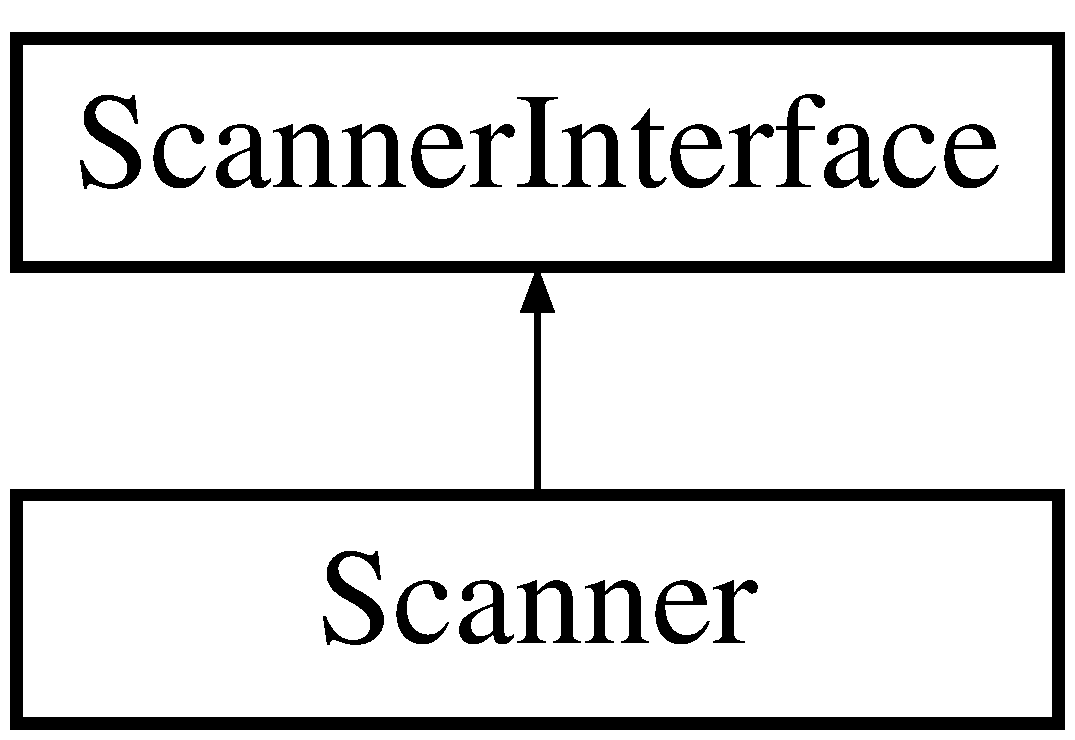
\includegraphics[height=2.000000cm]{classScannerInterface}
\end{center}
\end{figure}
\subsection*{Public Member Functions}
\begin{DoxyCompactItemize}
\item 
\mbox{\Hypertarget{classScannerInterface_a6e56474f9979ef6c66a614f0991a9f99}\label{classScannerInterface_a6e56474f9979ef6c66a614f0991a9f99}} 
\hyperlink{classScannerInterface_a6e56474f9979ef6c66a614f0991a9f99}{Scanner\+Interface} ()
\begin{DoxyCompactList}\small\item\em Construct a new \hyperlink{classScanner}{Scanner} Interface object of abstract class. \end{DoxyCompactList}\item 
\mbox{\Hypertarget{classScannerInterface_a25be999ce7d92de86814631974a96999}\label{classScannerInterface_a25be999ce7d92de86814631974a96999}} 
\hyperlink{classScannerInterface_a25be999ce7d92de86814631974a96999}{$\sim$\+Scanner\+Interface} ()
\begin{DoxyCompactList}\small\item\em Destroy the \hyperlink{classScanner}{Scanner} Interface object of the abstract class. \end{DoxyCompactList}\item 
virtual void \hyperlink{classScannerInterface_a32a25bd134d2d346e3652eea3180ea7b}{reset\+Data} ()=0
\begin{DoxyCompactList}\small\item\em Virtual function to reset all the acquired data. \end{DoxyCompactList}\item 
virtual std\+::vector$<$ double $>$ \hyperlink{classScannerInterface_a7f6b7a9cd907c8fdde13784ae3caec00}{get\+Object\+Velocity} ()=0
\begin{DoxyCompactList}\small\item\em Get the Object Velocity of the target as Scalar. \end{DoxyCompactList}\item 
virtual std\+::vector$<$ std\+::pair$<$ double, double $>$ $>$ \hyperlink{classScannerInterface_a526bd963b27ac01be5844bfcb9ecdb27}{get\+Target} ()=0
\begin{DoxyCompactList}\small\item\em Get the Target object in x and y coordinates based on a given plane. \end{DoxyCompactList}\item 
virtual std\+::vector$<$ std\+::pair$<$ double, double $>$ $>$ \hyperlink{classScannerInterface_a9dce1c9696b08fc10a1db681a479b0a9}{get\+Velocity\+Vector} ()=0
\begin{DoxyCompactList}\small\item\em Get the Velocity Vector object. \end{DoxyCompactList}\item 
virtual std\+::vector$<$ std\+::pair$<$ double, double $>$ $>$ \hyperlink{classScannerInterface_a27f991c8667a4c2524580addd264ae70}{get\+Predicted\+Target} ()=0
\begin{DoxyCompactList}\small\item\em Get the Predicted Target object. \end{DoxyCompactList}\end{DoxyCompactItemize}


\subsection{Detailed Description}
This \hyperlink{classScannerInterface}{Scanner\+Interface} is an abstract class that will be the base for multiple scanning classes. 

\begin{DoxySeeAlso}{See also}
\hyperlink{ScannerInterface_8h}{Scanner\+Interface.\+h} 
\end{DoxySeeAlso}


\subsection{Member Function Documentation}
\mbox{\Hypertarget{classScannerInterface_a7f6b7a9cd907c8fdde13784ae3caec00}\label{classScannerInterface_a7f6b7a9cd907c8fdde13784ae3caec00}} 
\index{Scanner\+Interface@{Scanner\+Interface}!get\+Object\+Velocity@{get\+Object\+Velocity}}
\index{get\+Object\+Velocity@{get\+Object\+Velocity}!Scanner\+Interface@{Scanner\+Interface}}
\subsubsection{\texorpdfstring{get\+Object\+Velocity()}{getObjectVelocity()}}
{\footnotesize\ttfamily virtual std\+::vector$<$double$>$ Scanner\+Interface\+::get\+Object\+Velocity (\begin{DoxyParamCaption}{ }\end{DoxyParamCaption})\hspace{0.3cm}{\ttfamily [pure virtual]}}



Get the Object Velocity of the target as Scalar. 

\begin{DoxyNote}{Note}
Will get the converted Scalar velocity of the vector 
\end{DoxyNote}
\begin{DoxyReturn}{Returns}
std\+::vector$<$double$>$ of velocity 
\end{DoxyReturn}


Implemented in \hyperlink{classScanner_ac9b03f1f8b6f38f6f8144affa6be9854}{Scanner}.

\mbox{\Hypertarget{classScannerInterface_a27f991c8667a4c2524580addd264ae70}\label{classScannerInterface_a27f991c8667a4c2524580addd264ae70}} 
\index{Scanner\+Interface@{Scanner\+Interface}!get\+Predicted\+Target@{get\+Predicted\+Target}}
\index{get\+Predicted\+Target@{get\+Predicted\+Target}!Scanner\+Interface@{Scanner\+Interface}}
\subsubsection{\texorpdfstring{get\+Predicted\+Target()}{getPredictedTarget()}}
{\footnotesize\ttfamily virtual std\+::vector$<$std\+::pair$<$double, double$>$ $>$ Scanner\+Interface\+::get\+Predicted\+Target (\begin{DoxyParamCaption}{ }\end{DoxyParamCaption})\hspace{0.3cm}{\ttfamily [pure virtual]}}



Get the Predicted Target object. 

\begin{DoxyNote}{Note}
Will get the predicted position in x and y 
\end{DoxyNote}
\begin{DoxyReturn}{Returns}
std\+::vector$<$std\+::pair$<$double, double$>$$>$ predicted\+\_\+position 
\end{DoxyReturn}


Implemented in \hyperlink{classScanner_a4f9ba72b2339cad7e3cb7ffe46196ea2}{Scanner}.

\mbox{\Hypertarget{classScannerInterface_a526bd963b27ac01be5844bfcb9ecdb27}\label{classScannerInterface_a526bd963b27ac01be5844bfcb9ecdb27}} 
\index{Scanner\+Interface@{Scanner\+Interface}!get\+Target@{get\+Target}}
\index{get\+Target@{get\+Target}!Scanner\+Interface@{Scanner\+Interface}}
\subsubsection{\texorpdfstring{get\+Target()}{getTarget()}}
{\footnotesize\ttfamily virtual std\+::vector$<$std\+::pair$<$double, double$>$ $>$ Scanner\+Interface\+::get\+Target (\begin{DoxyParamCaption}{ }\end{DoxyParamCaption})\hspace{0.3cm}{\ttfamily [pure virtual]}}



Get the Target object in x and y coordinates based on a given plane. 

\begin{DoxyNote}{Note}
Will be analysed in reference to a plane of reference 
\end{DoxyNote}
\begin{DoxyReturn}{Returns}
std\+::vector$<$std\+::pair$<$double, double$>$$>$ position 
\end{DoxyReturn}


Implemented in \hyperlink{classScanner_a556ac0598666bf9543099daef4655d6b}{Scanner}.

\mbox{\Hypertarget{classScannerInterface_a9dce1c9696b08fc10a1db681a479b0a9}\label{classScannerInterface_a9dce1c9696b08fc10a1db681a479b0a9}} 
\index{Scanner\+Interface@{Scanner\+Interface}!get\+Velocity\+Vector@{get\+Velocity\+Vector}}
\index{get\+Velocity\+Vector@{get\+Velocity\+Vector}!Scanner\+Interface@{Scanner\+Interface}}
\subsubsection{\texorpdfstring{get\+Velocity\+Vector()}{getVelocityVector()}}
{\footnotesize\ttfamily virtual std\+::vector$<$std\+::pair$<$double, double$>$ $>$ Scanner\+Interface\+::get\+Velocity\+Vector (\begin{DoxyParamCaption}{ }\end{DoxyParamCaption})\hspace{0.3cm}{\ttfamily [pure virtual]}}



Get the Velocity Vector object. 

\begin{DoxyNote}{Note}
The velocity will be obtain in rectangular coordiantes with Vx and Vy 
\end{DoxyNote}
\begin{DoxyReturn}{Returns}
std\+::vector$<$std\+::pair$<$double, double$>$$>$ velocity\+Vector 
\end{DoxyReturn}


Implemented in \hyperlink{classScanner_aa551cad3b1137f4fbe052181f09f987f}{Scanner}.

\mbox{\Hypertarget{classScannerInterface_a32a25bd134d2d346e3652eea3180ea7b}\label{classScannerInterface_a32a25bd134d2d346e3652eea3180ea7b}} 
\index{Scanner\+Interface@{Scanner\+Interface}!reset\+Data@{reset\+Data}}
\index{reset\+Data@{reset\+Data}!Scanner\+Interface@{Scanner\+Interface}}
\subsubsection{\texorpdfstring{reset\+Data()}{resetData()}}
{\footnotesize\ttfamily virtual void Scanner\+Interface\+::reset\+Data (\begin{DoxyParamCaption}{ }\end{DoxyParamCaption})\hspace{0.3cm}{\ttfamily [pure virtual]}}



Virtual function to reset all the acquired data. 

\begin{DoxyNote}{Note}
Will need to be used reset all the S\+TL containers of data 
\end{DoxyNote}


Implemented in \hyperlink{classScanner_a95dea82a0db3f7ca8cf5152c85f89239}{Scanner}.



The documentation for this class was generated from the following file\+:\begin{DoxyCompactItemize}
\item 
/home/esteban/git/pfms-\/2020a-\/esteban-\/andrade/scratch/\+Assignment3/\+Submission/a3/\hyperlink{ScannerInterface_8h}{Scanner\+Interface.\+h}\end{DoxyCompactItemize}

\hypertarget{classSimulator}{}\section{Simulator Class Reference}
\label{classSimulator}\index{Simulator@{Simulator}}
\subsection*{Public Member Functions}
\begin{DoxyCompactItemize}
\item 
\hyperlink{classSimulator_a62ab66763cb9e6cccbe88d45ab55547f}{Simulator} (void)
\begin{DoxyCompactList}\small\item\em \hyperlink{classSimulator}{Simulator} constructor. \end{DoxyCompactList}\item 
std\+::thread \hyperlink{classSimulator_a19ad57d2e32486e1cce2d8702060d930}{spawn} (void)
\begin{DoxyCompactList}\small\item\em Returns the simulation thread. \end{DoxyCompactList}\item 
\mbox{\Hypertarget{classSimulator_ae88ecc16eb03836e8b4a355836d7500b}\label{classSimulator_ae88ecc16eb03836e8b4a355836d7500b}} 
void \hyperlink{classSimulator_ae88ecc16eb03836e8b4a355836d7500b}{stop} (void)
\begin{DoxyCompactList}\small\item\em Stops the running simulation thread when invoked. \end{DoxyCompactList}\item 
long \hyperlink{classSimulator_acd0a0ca3e9d25ea92ffc05e14b77c5e6}{elapsed} (void)
\begin{DoxyCompactList}\small\item\em Gets the elapsed time since the simulation started. \end{DoxyCompactList}\item 
\hyperlink{structPose}{Pose} \hyperlink{classSimulator_ab498029a37713969af417acfa7208d08}{get\+Friendly\+Pose} (void)
\begin{DoxyCompactList}\small\item\em Return the friendly aircraft\textquotesingle{}s pose. \end{DoxyCompactList}\item 
double \hyperlink{classSimulator_a17d07e629ef87450d91d960c2e6b231e}{get\+Friendly\+Linear\+Velocity} (void)
\begin{DoxyCompactList}\small\item\em Return the friendly aircraft\textquotesingle{}s linear velocity. \end{DoxyCompactList}\item 
double \hyperlink{classSimulator_a054241a50cbf232b71acdaf4290855d3}{get\+Friendly\+Angular\+Velocity} (void)
\begin{DoxyCompactList}\small\item\em Return the friendly aircraft\textquotesingle{}s angular velocity. \end{DoxyCompactList}\item 
bool \hyperlink{classSimulator_adb1cff57466c3b03fd738036cb9cee63}{control\+Friendly} (double linear\+\_\+velocity, double angular\+\_\+velocity)
\begin{DoxyCompactList}\small\item\em Update the linear and angular velocity of the friendly aircraft. \end{DoxyCompactList}\item 
std\+::vector$<$ \hyperlink{structRangeVelocityStamped}{Range\+Velocity\+Stamped} $>$ \hyperlink{classSimulator_ae286a7571719440cc06b2441900efb44}{range\+Velocity\+To\+Bogies\+From\+Base} (void)
\begin{DoxyCompactList}\small\item\em Returns the range from the base station and velocity of bogies. \end{DoxyCompactList}\item 
std\+::vector$<$ \hyperlink{structRangeBearingStamped}{Range\+Bearing\+Stamped} $>$ \hyperlink{classSimulator_af78c417dd541bf1f671894f49739106f}{range\+Bearing\+To\+Bogies\+From\+Friendly} (void)
\begin{DoxyCompactList}\small\item\em Returns the range from the friendly aircraft to the bogie. \end{DoxyCompactList}\item 
void \hyperlink{classSimulator_aedf306bfd80a13ff07d9197bd5703805}{test\+Pose} (std\+::vector$<$ \hyperlink{structPose}{Pose} $>$ poses)
\begin{DoxyCompactList}\small\item\em Will render test aircraft by poses supplied within the airspace. \end{DoxyCompactList}\item 
double \hyperlink{classSimulator_ab21eff1f7776080c591765f099c2fb7e}{distance} (\hyperlink{structGlobalOrd}{Global\+Ord} o1, \hyperlink{structGlobalOrd}{Global\+Ord} o2)
\begin{DoxyCompactList}\small\item\em Calculates the euclidean distance between two coordiantes. \end{DoxyCompactList}\item 
\hyperlink{classSimulator_a62ab66763cb9e6cccbe88d45ab55547f}{Simulator} (void)
\begin{DoxyCompactList}\small\item\em \hyperlink{classSimulator}{Simulator} constructor. \end{DoxyCompactList}\item 
std\+::thread \hyperlink{classSimulator_a19ad57d2e32486e1cce2d8702060d930}{spawn} (void)
\begin{DoxyCompactList}\small\item\em Returns the simulation thread. \end{DoxyCompactList}\item 
\mbox{\Hypertarget{classSimulator_ae88ecc16eb03836e8b4a355836d7500b}\label{classSimulator_ae88ecc16eb03836e8b4a355836d7500b}} 
void \hyperlink{classSimulator_ae88ecc16eb03836e8b4a355836d7500b}{stop} (void)
\begin{DoxyCompactList}\small\item\em Stops the running simulation thread when invoked. \end{DoxyCompactList}\item 
long \hyperlink{classSimulator_acd0a0ca3e9d25ea92ffc05e14b77c5e6}{elapsed} (void)
\begin{DoxyCompactList}\small\item\em Gets the elapsed time since the simulation started. \end{DoxyCompactList}\item 
\hyperlink{structPose}{Pose} \hyperlink{classSimulator_ab498029a37713969af417acfa7208d08}{get\+Friendly\+Pose} (void)
\begin{DoxyCompactList}\small\item\em Return the friendly aircraft\textquotesingle{}s pose. \end{DoxyCompactList}\item 
double \hyperlink{classSimulator_a17d07e629ef87450d91d960c2e6b231e}{get\+Friendly\+Linear\+Velocity} (void)
\begin{DoxyCompactList}\small\item\em Return the friendly aircraft\textquotesingle{}s linear velocity. \end{DoxyCompactList}\item 
double \hyperlink{classSimulator_a054241a50cbf232b71acdaf4290855d3}{get\+Friendly\+Angular\+Velocity} (void)
\begin{DoxyCompactList}\small\item\em Return the friendly aircraft\textquotesingle{}s angular velocity. \end{DoxyCompactList}\item 
bool \hyperlink{classSimulator_adb1cff57466c3b03fd738036cb9cee63}{control\+Friendly} (double linear\+\_\+velocity, double angular\+\_\+velocity)
\begin{DoxyCompactList}\small\item\em Update the linear and angular velocity of the friendly aircraft. \end{DoxyCompactList}\item 
std\+::vector$<$ \hyperlink{structRangeVelocityStamped}{Range\+Velocity\+Stamped} $>$ \hyperlink{classSimulator_ae286a7571719440cc06b2441900efb44}{range\+Velocity\+To\+Bogies\+From\+Base} (void)
\begin{DoxyCompactList}\small\item\em Returns the range from the base station and velocity of bogies. \end{DoxyCompactList}\item 
std\+::vector$<$ \hyperlink{structRangeBearingStamped}{Range\+Bearing\+Stamped} $>$ \hyperlink{classSimulator_af78c417dd541bf1f671894f49739106f}{range\+Bearing\+To\+Bogies\+From\+Friendly} (void)
\begin{DoxyCompactList}\small\item\em Returns the range from the friendly aircraft to the bogie. \end{DoxyCompactList}\item 
void \hyperlink{classSimulator_aedf306bfd80a13ff07d9197bd5703805}{test\+Pose} (std\+::vector$<$ \hyperlink{structPose}{Pose} $>$ poses)
\begin{DoxyCompactList}\small\item\em Will render test aircraft by poses supplied within the airspace. \end{DoxyCompactList}\item 
double \hyperlink{classSimulator_ab21eff1f7776080c591765f099c2fb7e}{distance} (\hyperlink{structGlobalOrd}{Global\+Ord} o1, \hyperlink{structGlobalOrd}{Global\+Ord} o2)
\begin{DoxyCompactList}\small\item\em Calculates the euclidean distance between two coordiantes. \end{DoxyCompactList}\end{DoxyCompactItemize}
\subsection*{Public Attributes}
\begin{DoxyCompactItemize}
\item 
const std\+::string \hyperlink{classSimulator_a4eea5ab08ac7b24af87b81d8babad136}{library\+\_\+version} = \char`\"{}Version 20.\+5.\+16\char`\"{}
\end{DoxyCompactItemize}
\subsection*{Static Public Attributes}
\begin{DoxyCompactItemize}
\item 
static const double \hyperlink{classSimulator_a8250a5fd76149109333aed2c91fa846e}{V\+\_\+\+T\+E\+RM}
\item 
static const unsigned int \hyperlink{classSimulator_a95d27d8bc5a3dd5a67aeba981128ba4e}{M\+A\+X\+\_\+G}
\item 
static const double \hyperlink{classSimulator_aa4e6371b6605ae050de558167256a9d0}{M\+A\+X\+\_\+V}
\item 
static const double \hyperlink{classSimulator_a5f06c727e635ea9229cb12f662d05036}{A\+I\+R\+S\+P\+A\+C\+E\+\_\+\+S\+I\+ZE}
\item 
static const \hyperlink{structGlobalOrd}{Global\+Ord} \hyperlink{classSimulator_a21f23eb0363ffc0a9cc438e0249f8968}{B\+S\+T\+A\+T\+I\+O\+N\+\_\+\+L\+OC}
\item 
static const unsigned int \hyperlink{classSimulator_a4ecdf564a4773968f2c2acc4f9bad29f}{B\+S\+T\+A\+T\+I\+O\+N\+\_\+\+R\+E\+F\+\_\+\+R\+A\+TE}
\item 
static const unsigned int \hyperlink{classSimulator_a4936b9aff3bee55866a520bf36b4fb5a}{F\+R\+I\+E\+N\+D\+L\+Y\+\_\+\+R\+E\+F\+\_\+\+R\+A\+TE}
\end{DoxyCompactItemize}


\subsection{Constructor \& Destructor Documentation}
\mbox{\Hypertarget{classSimulator_a62ab66763cb9e6cccbe88d45ab55547f}\label{classSimulator_a62ab66763cb9e6cccbe88d45ab55547f}} 
\index{Simulator@{Simulator}!Simulator@{Simulator}}
\index{Simulator@{Simulator}!Simulator@{Simulator}}
\subsubsection{\texorpdfstring{Simulator()}{Simulator()}\hspace{0.1cm}{\footnotesize\ttfamily [1/2]}}
{\footnotesize\ttfamily Simulator\+::\+Simulator (\begin{DoxyParamCaption}\item[{void}]{ }\end{DoxyParamCaption})}



\hyperlink{classSimulator}{Simulator} constructor. 

Will randomly intialise the position of the bogie and friendly within the airspace. \mbox{\Hypertarget{classSimulator_a62ab66763cb9e6cccbe88d45ab55547f}\label{classSimulator_a62ab66763cb9e6cccbe88d45ab55547f}} 
\index{Simulator@{Simulator}!Simulator@{Simulator}}
\index{Simulator@{Simulator}!Simulator@{Simulator}}
\subsubsection{\texorpdfstring{Simulator()}{Simulator()}\hspace{0.1cm}{\footnotesize\ttfamily [2/2]}}
{\footnotesize\ttfamily Simulator\+::\+Simulator (\begin{DoxyParamCaption}\item[{void}]{ }\end{DoxyParamCaption})}



\hyperlink{classSimulator}{Simulator} constructor. 

Will randomly intialise the position of the bogie and friendly within the airspace. 

\subsection{Member Function Documentation}
\mbox{\Hypertarget{classSimulator_adb1cff57466c3b03fd738036cb9cee63}\label{classSimulator_adb1cff57466c3b03fd738036cb9cee63}} 
\index{Simulator@{Simulator}!control\+Friendly@{control\+Friendly}}
\index{control\+Friendly@{control\+Friendly}!Simulator@{Simulator}}
\subsubsection{\texorpdfstring{control\+Friendly()}{controlFriendly()}\hspace{0.1cm}{\footnotesize\ttfamily [1/2]}}
{\footnotesize\ttfamily bool Simulator\+::control\+Friendly (\begin{DoxyParamCaption}\item[{double}]{linear\+\_\+velocity,  }\item[{double}]{angular\+\_\+velocity }\end{DoxyParamCaption})}



Update the linear and angular velocity of the friendly aircraft. 


\begin{DoxyParams}{Parameters}
{\em linear\+\_\+velocity} & The linear velocity of the aircraft (metres/second) \\
\hline
{\em angular\+\_\+velocity} & The angular velocity of the aircraft (radians/second)\\
\hline
\end{DoxyParams}
\begin{DoxyReturn}{Returns}
bool -\/ Will return false if the calculated gforce is more than 6G\textquotesingle{}s OR if the linear velocity is less than the terminal OR the linear velocity is more than the max. 
\end{DoxyReturn}
\mbox{\Hypertarget{classSimulator_adb1cff57466c3b03fd738036cb9cee63}\label{classSimulator_adb1cff57466c3b03fd738036cb9cee63}} 
\index{Simulator@{Simulator}!control\+Friendly@{control\+Friendly}}
\index{control\+Friendly@{control\+Friendly}!Simulator@{Simulator}}
\subsubsection{\texorpdfstring{control\+Friendly()}{controlFriendly()}\hspace{0.1cm}{\footnotesize\ttfamily [2/2]}}
{\footnotesize\ttfamily bool Simulator\+::control\+Friendly (\begin{DoxyParamCaption}\item[{double}]{linear\+\_\+velocity,  }\item[{double}]{angular\+\_\+velocity }\end{DoxyParamCaption})}



Update the linear and angular velocity of the friendly aircraft. 


\begin{DoxyParams}{Parameters}
{\em linear\+\_\+velocity} & The linear velocity of the aircraft (metres/second) \\
\hline
{\em angular\+\_\+velocity} & The angular velocity of the aircraft (radians/second)\\
\hline
\end{DoxyParams}
\begin{DoxyReturn}{Returns}
bool -\/ Will return false if the calculated gforce is more than 6G\textquotesingle{}s OR if the linear velocity is less than the terminal OR the linear velocity is more than the max. 
\end{DoxyReturn}
\mbox{\Hypertarget{classSimulator_ab21eff1f7776080c591765f099c2fb7e}\label{classSimulator_ab21eff1f7776080c591765f099c2fb7e}} 
\index{Simulator@{Simulator}!distance@{distance}}
\index{distance@{distance}!Simulator@{Simulator}}
\subsubsection{\texorpdfstring{distance()}{distance()}\hspace{0.1cm}{\footnotesize\ttfamily [1/2]}}
{\footnotesize\ttfamily double Simulator\+::distance (\begin{DoxyParamCaption}\item[{\hyperlink{structGlobalOrd}{Global\+Ord}}]{o1,  }\item[{\hyperlink{structGlobalOrd}{Global\+Ord}}]{o2 }\end{DoxyParamCaption})}



Calculates the euclidean distance between two coordiantes. 


\begin{DoxyParams}{Parameters}
{\em o1} & The first coordinate. \\
\hline
{\em o2} & The second coordinate. \\
\hline
\end{DoxyParams}
\begin{DoxyReturn}{Returns}
double -\/ The distance between the two coordiantes. 
\end{DoxyReturn}
\mbox{\Hypertarget{classSimulator_ab21eff1f7776080c591765f099c2fb7e}\label{classSimulator_ab21eff1f7776080c591765f099c2fb7e}} 
\index{Simulator@{Simulator}!distance@{distance}}
\index{distance@{distance}!Simulator@{Simulator}}
\subsubsection{\texorpdfstring{distance()}{distance()}\hspace{0.1cm}{\footnotesize\ttfamily [2/2]}}
{\footnotesize\ttfamily double Simulator\+::distance (\begin{DoxyParamCaption}\item[{\hyperlink{structGlobalOrd}{Global\+Ord}}]{o1,  }\item[{\hyperlink{structGlobalOrd}{Global\+Ord}}]{o2 }\end{DoxyParamCaption})}



Calculates the euclidean distance between two coordiantes. 


\begin{DoxyParams}{Parameters}
{\em o1} & The first coordinate. \\
\hline
{\em o2} & The second coordinate. \\
\hline
\end{DoxyParams}
\begin{DoxyReturn}{Returns}
double -\/ The distance between the two coordiantes. 
\end{DoxyReturn}
\mbox{\Hypertarget{classSimulator_acd0a0ca3e9d25ea92ffc05e14b77c5e6}\label{classSimulator_acd0a0ca3e9d25ea92ffc05e14b77c5e6}} 
\index{Simulator@{Simulator}!elapsed@{elapsed}}
\index{elapsed@{elapsed}!Simulator@{Simulator}}
\subsubsection{\texorpdfstring{elapsed()}{elapsed()}\hspace{0.1cm}{\footnotesize\ttfamily [1/2]}}
{\footnotesize\ttfamily long Simulator\+::elapsed (\begin{DoxyParamCaption}\item[{void}]{ }\end{DoxyParamCaption})}



Gets the elapsed time since the simulation started. 

\begin{DoxyReturn}{Returns}
long -\/ The elapsed time in milliseconds. 
\end{DoxyReturn}
\mbox{\Hypertarget{classSimulator_acd0a0ca3e9d25ea92ffc05e14b77c5e6}\label{classSimulator_acd0a0ca3e9d25ea92ffc05e14b77c5e6}} 
\index{Simulator@{Simulator}!elapsed@{elapsed}}
\index{elapsed@{elapsed}!Simulator@{Simulator}}
\subsubsection{\texorpdfstring{elapsed()}{elapsed()}\hspace{0.1cm}{\footnotesize\ttfamily [2/2]}}
{\footnotesize\ttfamily long Simulator\+::elapsed (\begin{DoxyParamCaption}\item[{void}]{ }\end{DoxyParamCaption})}



Gets the elapsed time since the simulation started. 

\begin{DoxyReturn}{Returns}
long -\/ The elapsed time in milliseconds. 
\end{DoxyReturn}
\mbox{\Hypertarget{classSimulator_a054241a50cbf232b71acdaf4290855d3}\label{classSimulator_a054241a50cbf232b71acdaf4290855d3}} 
\index{Simulator@{Simulator}!get\+Friendly\+Angular\+Velocity@{get\+Friendly\+Angular\+Velocity}}
\index{get\+Friendly\+Angular\+Velocity@{get\+Friendly\+Angular\+Velocity}!Simulator@{Simulator}}
\subsubsection{\texorpdfstring{get\+Friendly\+Angular\+Velocity()}{getFriendlyAngularVelocity()}\hspace{0.1cm}{\footnotesize\ttfamily [1/2]}}
{\footnotesize\ttfamily double Simulator\+::get\+Friendly\+Angular\+Velocity (\begin{DoxyParamCaption}\item[{void}]{ }\end{DoxyParamCaption})}



Return the friendly aircraft\textquotesingle{}s angular velocity. 

\begin{DoxyReturn}{Returns}
double -\/ The aircraft\textquotesingle{}s angular velocity (radians/second). 
\end{DoxyReturn}
\mbox{\Hypertarget{classSimulator_a054241a50cbf232b71acdaf4290855d3}\label{classSimulator_a054241a50cbf232b71acdaf4290855d3}} 
\index{Simulator@{Simulator}!get\+Friendly\+Angular\+Velocity@{get\+Friendly\+Angular\+Velocity}}
\index{get\+Friendly\+Angular\+Velocity@{get\+Friendly\+Angular\+Velocity}!Simulator@{Simulator}}
\subsubsection{\texorpdfstring{get\+Friendly\+Angular\+Velocity()}{getFriendlyAngularVelocity()}\hspace{0.1cm}{\footnotesize\ttfamily [2/2]}}
{\footnotesize\ttfamily double Simulator\+::get\+Friendly\+Angular\+Velocity (\begin{DoxyParamCaption}\item[{void}]{ }\end{DoxyParamCaption})}



Return the friendly aircraft\textquotesingle{}s angular velocity. 

\begin{DoxyReturn}{Returns}
double -\/ The aircraft\textquotesingle{}s angular velocity (radians/second). 
\end{DoxyReturn}
\mbox{\Hypertarget{classSimulator_a17d07e629ef87450d91d960c2e6b231e}\label{classSimulator_a17d07e629ef87450d91d960c2e6b231e}} 
\index{Simulator@{Simulator}!get\+Friendly\+Linear\+Velocity@{get\+Friendly\+Linear\+Velocity}}
\index{get\+Friendly\+Linear\+Velocity@{get\+Friendly\+Linear\+Velocity}!Simulator@{Simulator}}
\subsubsection{\texorpdfstring{get\+Friendly\+Linear\+Velocity()}{getFriendlyLinearVelocity()}\hspace{0.1cm}{\footnotesize\ttfamily [1/2]}}
{\footnotesize\ttfamily double Simulator\+::get\+Friendly\+Linear\+Velocity (\begin{DoxyParamCaption}\item[{void}]{ }\end{DoxyParamCaption})}



Return the friendly aircraft\textquotesingle{}s linear velocity. 

\begin{DoxyReturn}{Returns}
double -\/ The aircraft\textquotesingle{}s linear velocity (metres/second). 
\end{DoxyReturn}
\mbox{\Hypertarget{classSimulator_a17d07e629ef87450d91d960c2e6b231e}\label{classSimulator_a17d07e629ef87450d91d960c2e6b231e}} 
\index{Simulator@{Simulator}!get\+Friendly\+Linear\+Velocity@{get\+Friendly\+Linear\+Velocity}}
\index{get\+Friendly\+Linear\+Velocity@{get\+Friendly\+Linear\+Velocity}!Simulator@{Simulator}}
\subsubsection{\texorpdfstring{get\+Friendly\+Linear\+Velocity()}{getFriendlyLinearVelocity()}\hspace{0.1cm}{\footnotesize\ttfamily [2/2]}}
{\footnotesize\ttfamily double Simulator\+::get\+Friendly\+Linear\+Velocity (\begin{DoxyParamCaption}\item[{void}]{ }\end{DoxyParamCaption})}



Return the friendly aircraft\textquotesingle{}s linear velocity. 

\begin{DoxyReturn}{Returns}
double -\/ The aircraft\textquotesingle{}s linear velocity (metres/second). 
\end{DoxyReturn}
\mbox{\Hypertarget{classSimulator_ab498029a37713969af417acfa7208d08}\label{classSimulator_ab498029a37713969af417acfa7208d08}} 
\index{Simulator@{Simulator}!get\+Friendly\+Pose@{get\+Friendly\+Pose}}
\index{get\+Friendly\+Pose@{get\+Friendly\+Pose}!Simulator@{Simulator}}
\subsubsection{\texorpdfstring{get\+Friendly\+Pose()}{getFriendlyPose()}\hspace{0.1cm}{\footnotesize\ttfamily [1/2]}}
{\footnotesize\ttfamily \hyperlink{structPose}{Pose} Simulator\+::get\+Friendly\+Pose (\begin{DoxyParamCaption}\item[{void}]{ }\end{DoxyParamCaption})}



Return the friendly aircraft\textquotesingle{}s pose. 

\begin{DoxyReturn}{Returns}
\hyperlink{structPose}{Pose} -\/ The aircraft\textquotesingle{}s x, y position (metres) and orientation (radians). 
\end{DoxyReturn}
\mbox{\Hypertarget{classSimulator_ab498029a37713969af417acfa7208d08}\label{classSimulator_ab498029a37713969af417acfa7208d08}} 
\index{Simulator@{Simulator}!get\+Friendly\+Pose@{get\+Friendly\+Pose}}
\index{get\+Friendly\+Pose@{get\+Friendly\+Pose}!Simulator@{Simulator}}
\subsubsection{\texorpdfstring{get\+Friendly\+Pose()}{getFriendlyPose()}\hspace{0.1cm}{\footnotesize\ttfamily [2/2]}}
{\footnotesize\ttfamily \hyperlink{structPose}{Pose} Simulator\+::get\+Friendly\+Pose (\begin{DoxyParamCaption}\item[{void}]{ }\end{DoxyParamCaption})}



Return the friendly aircraft\textquotesingle{}s pose. 

\begin{DoxyReturn}{Returns}
\hyperlink{structPose}{Pose} -\/ The aircraft\textquotesingle{}s x, y position (metres) and orientation (radians). 
\end{DoxyReturn}
\mbox{\Hypertarget{classSimulator_af78c417dd541bf1f671894f49739106f}\label{classSimulator_af78c417dd541bf1f671894f49739106f}} 
\index{Simulator@{Simulator}!range\+Bearing\+To\+Bogies\+From\+Friendly@{range\+Bearing\+To\+Bogies\+From\+Friendly}}
\index{range\+Bearing\+To\+Bogies\+From\+Friendly@{range\+Bearing\+To\+Bogies\+From\+Friendly}!Simulator@{Simulator}}
\subsubsection{\texorpdfstring{range\+Bearing\+To\+Bogies\+From\+Friendly()}{rangeBearingToBogiesFromFriendly()}\hspace{0.1cm}{\footnotesize\ttfamily [1/2]}}
{\footnotesize\ttfamily std\+::vector$<$\hyperlink{structRangeBearingStamped}{Range\+Bearing\+Stamped}$>$ Simulator\+::range\+Bearing\+To\+Bogies\+From\+Friendly (\begin{DoxyParamCaption}\item[{void}]{ }\end{DoxyParamCaption})}



Returns the range from the friendly aircraft to the bogie. 

\begin{DoxyReturn}{Returns}
Range\+Stamped -\/ The range and bearing from friendly to bogies (metres) (rad), with a timestamp (milliseconds). 
\end{DoxyReturn}
\begin{DoxyNote}{Note}
This function will perform a sleep(\+F\+R\+I\+E\+N\+D\+L\+Y\+\_\+\+R\+E\+F\+R\+E\+S\+H\+\_\+\+R\+A\+T\+E), to enforce the refresh rate of the friendly aircraft. 

The timestamp uses the simulation epoch timer as a reference. 
\end{DoxyNote}
\mbox{\Hypertarget{classSimulator_af78c417dd541bf1f671894f49739106f}\label{classSimulator_af78c417dd541bf1f671894f49739106f}} 
\index{Simulator@{Simulator}!range\+Bearing\+To\+Bogies\+From\+Friendly@{range\+Bearing\+To\+Bogies\+From\+Friendly}}
\index{range\+Bearing\+To\+Bogies\+From\+Friendly@{range\+Bearing\+To\+Bogies\+From\+Friendly}!Simulator@{Simulator}}
\subsubsection{\texorpdfstring{range\+Bearing\+To\+Bogies\+From\+Friendly()}{rangeBearingToBogiesFromFriendly()}\hspace{0.1cm}{\footnotesize\ttfamily [2/2]}}
{\footnotesize\ttfamily std\+::vector$<$\hyperlink{structRangeBearingStamped}{Range\+Bearing\+Stamped}$>$ Simulator\+::range\+Bearing\+To\+Bogies\+From\+Friendly (\begin{DoxyParamCaption}\item[{void}]{ }\end{DoxyParamCaption})}



Returns the range from the friendly aircraft to the bogie. 

\begin{DoxyReturn}{Returns}
Range\+Stamped -\/ The range and bearing from friendly to bogies (metres) (rad), with a timestamp (milliseconds). 
\end{DoxyReturn}
\begin{DoxyNote}{Note}
This function will perform a sleep(\+F\+R\+I\+E\+N\+D\+L\+Y\+\_\+\+R\+E\+F\+R\+E\+S\+H\+\_\+\+R\+A\+T\+E), to enforce the refresh rate of the friendly aircraft. 

The timestamp uses the simulation epoch timer as a reference. 
\end{DoxyNote}
\mbox{\Hypertarget{classSimulator_ae286a7571719440cc06b2441900efb44}\label{classSimulator_ae286a7571719440cc06b2441900efb44}} 
\index{Simulator@{Simulator}!range\+Velocity\+To\+Bogies\+From\+Base@{range\+Velocity\+To\+Bogies\+From\+Base}}
\index{range\+Velocity\+To\+Bogies\+From\+Base@{range\+Velocity\+To\+Bogies\+From\+Base}!Simulator@{Simulator}}
\subsubsection{\texorpdfstring{range\+Velocity\+To\+Bogies\+From\+Base()}{rangeVelocityToBogiesFromBase()}\hspace{0.1cm}{\footnotesize\ttfamily [1/2]}}
{\footnotesize\ttfamily std\+::vector$<$\hyperlink{structRangeVelocityStamped}{Range\+Velocity\+Stamped}$>$ Simulator\+::range\+Velocity\+To\+Bogies\+From\+Base (\begin{DoxyParamCaption}\item[{void}]{ }\end{DoxyParamCaption})}



Returns the range from the base station and velocity of bogies. 

\begin{DoxyReturn}{Returns}
\hyperlink{structRangeVelocityStamped}{Range\+Velocity\+Stamped} -\/ The range from bogie to base (metres), and the velocity of bogie (m/s) with a timestamp (milliseconds). 
\end{DoxyReturn}
\begin{DoxyNote}{Note}
This function will perform a sleep(\+B\+A\+S\+E\+\_\+\+S\+T\+A\+T\+I\+O\+N\+\_\+\+R\+E\+F\+R\+E\+S\+H\+\_\+\+R\+A\+T\+E), to enforce the refresh rate of the friendly aircraft. 

The timestamp uses the simulation epoch timer as a reference. 
\end{DoxyNote}
\mbox{\Hypertarget{classSimulator_ae286a7571719440cc06b2441900efb44}\label{classSimulator_ae286a7571719440cc06b2441900efb44}} 
\index{Simulator@{Simulator}!range\+Velocity\+To\+Bogies\+From\+Base@{range\+Velocity\+To\+Bogies\+From\+Base}}
\index{range\+Velocity\+To\+Bogies\+From\+Base@{range\+Velocity\+To\+Bogies\+From\+Base}!Simulator@{Simulator}}
\subsubsection{\texorpdfstring{range\+Velocity\+To\+Bogies\+From\+Base()}{rangeVelocityToBogiesFromBase()}\hspace{0.1cm}{\footnotesize\ttfamily [2/2]}}
{\footnotesize\ttfamily std\+::vector$<$\hyperlink{structRangeVelocityStamped}{Range\+Velocity\+Stamped}$>$ Simulator\+::range\+Velocity\+To\+Bogies\+From\+Base (\begin{DoxyParamCaption}\item[{void}]{ }\end{DoxyParamCaption})}



Returns the range from the base station and velocity of bogies. 

\begin{DoxyReturn}{Returns}
\hyperlink{structRangeVelocityStamped}{Range\+Velocity\+Stamped} -\/ The range from bogie to base (metres), and the velocity of bogie (m/s) with a timestamp (milliseconds). 
\end{DoxyReturn}
\begin{DoxyNote}{Note}
This function will perform a sleep(\+B\+A\+S\+E\+\_\+\+S\+T\+A\+T\+I\+O\+N\+\_\+\+R\+E\+F\+R\+E\+S\+H\+\_\+\+R\+A\+T\+E), to enforce the refresh rate of the friendly aircraft. 

The timestamp uses the simulation epoch timer as a reference. 
\end{DoxyNote}
\mbox{\Hypertarget{classSimulator_a19ad57d2e32486e1cce2d8702060d930}\label{classSimulator_a19ad57d2e32486e1cce2d8702060d930}} 
\index{Simulator@{Simulator}!spawn@{spawn}}
\index{spawn@{spawn}!Simulator@{Simulator}}
\subsubsection{\texorpdfstring{spawn()}{spawn()}\hspace{0.1cm}{\footnotesize\ttfamily [1/2]}}
{\footnotesize\ttfamily std\+::thread Simulator\+::spawn (\begin{DoxyParamCaption}\item[{void}]{ }\end{DoxyParamCaption})}



Returns the simulation thread. 

\begin{DoxyNote}{Note}
This thread will terminate if {\ttfamily \hyperlink{classSimulator_ae88ecc16eb03836e8b4a355836d7500b}{stop()}} is called OR, the user has not supplied control to the friendly aircraft within a timely manner 
\end{DoxyNote}
\mbox{\Hypertarget{classSimulator_a19ad57d2e32486e1cce2d8702060d930}\label{classSimulator_a19ad57d2e32486e1cce2d8702060d930}} 
\index{Simulator@{Simulator}!spawn@{spawn}}
\index{spawn@{spawn}!Simulator@{Simulator}}
\subsubsection{\texorpdfstring{spawn()}{spawn()}\hspace{0.1cm}{\footnotesize\ttfamily [2/2]}}
{\footnotesize\ttfamily std\+::thread Simulator\+::spawn (\begin{DoxyParamCaption}\item[{void}]{ }\end{DoxyParamCaption})}



Returns the simulation thread. 

\begin{DoxyNote}{Note}
This thread will terminate if {\ttfamily \hyperlink{classSimulator_ae88ecc16eb03836e8b4a355836d7500b}{stop()}} is called OR, the user has not supplied control to the friendly aircraft within a timely manner 
\end{DoxyNote}
\mbox{\Hypertarget{classSimulator_aedf306bfd80a13ff07d9197bd5703805}\label{classSimulator_aedf306bfd80a13ff07d9197bd5703805}} 
\index{Simulator@{Simulator}!test\+Pose@{test\+Pose}}
\index{test\+Pose@{test\+Pose}!Simulator@{Simulator}}
\subsubsection{\texorpdfstring{test\+Pose()}{testPose()}\hspace{0.1cm}{\footnotesize\ttfamily [1/2]}}
{\footnotesize\ttfamily void Simulator\+::test\+Pose (\begin{DoxyParamCaption}\item[{std\+::vector$<$ \hyperlink{structPose}{Pose} $>$}]{poses }\end{DoxyParamCaption})}



Will render test aircraft by poses supplied within the airspace. 

Callers may use this method to draw additional aircraft within the airspace for testing purposes. It will stay on screen for 1 second.


\begin{DoxyParams}{Parameters}
{\em pose} & The pose to display. \\
\hline
\end{DoxyParams}
\mbox{\Hypertarget{classSimulator_aedf306bfd80a13ff07d9197bd5703805}\label{classSimulator_aedf306bfd80a13ff07d9197bd5703805}} 
\index{Simulator@{Simulator}!test\+Pose@{test\+Pose}}
\index{test\+Pose@{test\+Pose}!Simulator@{Simulator}}
\subsubsection{\texorpdfstring{test\+Pose()}{testPose()}\hspace{0.1cm}{\footnotesize\ttfamily [2/2]}}
{\footnotesize\ttfamily void Simulator\+::test\+Pose (\begin{DoxyParamCaption}\item[{std\+::vector$<$ \hyperlink{structPose}{Pose} $>$}]{poses }\end{DoxyParamCaption})}



Will render test aircraft by poses supplied within the airspace. 

Callers may use this method to draw additional aircraft within the airspace for testing purposes. It will stay on screen for 1 second.


\begin{DoxyParams}{Parameters}
{\em pose} & The pose to display. \\
\hline
\end{DoxyParams}


\subsection{Member Data Documentation}
\mbox{\Hypertarget{classSimulator_a5f06c727e635ea9229cb12f662d05036}\label{classSimulator_a5f06c727e635ea9229cb12f662d05036}} 
\index{Simulator@{Simulator}!A\+I\+R\+S\+P\+A\+C\+E\+\_\+\+S\+I\+ZE@{A\+I\+R\+S\+P\+A\+C\+E\+\_\+\+S\+I\+ZE}}
\index{A\+I\+R\+S\+P\+A\+C\+E\+\_\+\+S\+I\+ZE@{A\+I\+R\+S\+P\+A\+C\+E\+\_\+\+S\+I\+ZE}!Simulator@{Simulator}}
\subsubsection{\texorpdfstring{A\+I\+R\+S\+P\+A\+C\+E\+\_\+\+S\+I\+ZE}{AIRSPACE\_SIZE}}
{\footnotesize\ttfamily static const double Simulator\+::\+A\+I\+R\+S\+P\+A\+C\+E\+\_\+\+S\+I\+ZE\hspace{0.3cm}{\ttfamily [static]}}

The airspace size is (A\+I\+R\+S\+P\+A\+C\+E\+\_\+\+S\+I\+ZE x A\+I\+R\+S\+P\+A\+C\+E\+\_\+\+S\+I\+ZE) in metres \mbox{\Hypertarget{classSimulator_a21f23eb0363ffc0a9cc438e0249f8968}\label{classSimulator_a21f23eb0363ffc0a9cc438e0249f8968}} 
\index{Simulator@{Simulator}!B\+S\+T\+A\+T\+I\+O\+N\+\_\+\+L\+OC@{B\+S\+T\+A\+T\+I\+O\+N\+\_\+\+L\+OC}}
\index{B\+S\+T\+A\+T\+I\+O\+N\+\_\+\+L\+OC@{B\+S\+T\+A\+T\+I\+O\+N\+\_\+\+L\+OC}!Simulator@{Simulator}}
\subsubsection{\texorpdfstring{B\+S\+T\+A\+T\+I\+O\+N\+\_\+\+L\+OC}{BSTATION\_LOC}}
{\footnotesize\ttfamily static const \hyperlink{structGlobalOrd}{Global\+Ord} Simulator\+::\+B\+S\+T\+A\+T\+I\+O\+N\+\_\+\+L\+OC\hspace{0.3cm}{\ttfamily [static]}}

The location of the base station \mbox{\Hypertarget{classSimulator_a4ecdf564a4773968f2c2acc4f9bad29f}\label{classSimulator_a4ecdf564a4773968f2c2acc4f9bad29f}} 
\index{Simulator@{Simulator}!B\+S\+T\+A\+T\+I\+O\+N\+\_\+\+R\+E\+F\+\_\+\+R\+A\+TE@{B\+S\+T\+A\+T\+I\+O\+N\+\_\+\+R\+E\+F\+\_\+\+R\+A\+TE}}
\index{B\+S\+T\+A\+T\+I\+O\+N\+\_\+\+R\+E\+F\+\_\+\+R\+A\+TE@{B\+S\+T\+A\+T\+I\+O\+N\+\_\+\+R\+E\+F\+\_\+\+R\+A\+TE}!Simulator@{Simulator}}
\subsubsection{\texorpdfstring{B\+S\+T\+A\+T\+I\+O\+N\+\_\+\+R\+E\+F\+\_\+\+R\+A\+TE}{BSTATION\_REF\_RATE}}
{\footnotesize\ttfamily static const unsigned int Simulator\+::\+B\+S\+T\+A\+T\+I\+O\+N\+\_\+\+R\+E\+F\+\_\+\+R\+A\+TE\hspace{0.3cm}{\ttfamily [static]}}

The rate (milliseconds) at which the base station produces range to bogie \mbox{\Hypertarget{classSimulator_a4936b9aff3bee55866a520bf36b4fb5a}\label{classSimulator_a4936b9aff3bee55866a520bf36b4fb5a}} 
\index{Simulator@{Simulator}!F\+R\+I\+E\+N\+D\+L\+Y\+\_\+\+R\+E\+F\+\_\+\+R\+A\+TE@{F\+R\+I\+E\+N\+D\+L\+Y\+\_\+\+R\+E\+F\+\_\+\+R\+A\+TE}}
\index{F\+R\+I\+E\+N\+D\+L\+Y\+\_\+\+R\+E\+F\+\_\+\+R\+A\+TE@{F\+R\+I\+E\+N\+D\+L\+Y\+\_\+\+R\+E\+F\+\_\+\+R\+A\+TE}!Simulator@{Simulator}}
\subsubsection{\texorpdfstring{F\+R\+I\+E\+N\+D\+L\+Y\+\_\+\+R\+E\+F\+\_\+\+R\+A\+TE}{FRIENDLY\_REF\_RATE}}
{\footnotesize\ttfamily static const unsigned int Simulator\+::\+F\+R\+I\+E\+N\+D\+L\+Y\+\_\+\+R\+E\+F\+\_\+\+R\+A\+TE\hspace{0.3cm}{\ttfamily [static]}}

The rate (milliseconds) at which the friendly produces range to bogie \mbox{\Hypertarget{classSimulator_a4eea5ab08ac7b24af87b81d8babad136}\label{classSimulator_a4eea5ab08ac7b24af87b81d8babad136}} 
\index{Simulator@{Simulator}!library\+\_\+version@{library\+\_\+version}}
\index{library\+\_\+version@{library\+\_\+version}!Simulator@{Simulator}}
\subsubsection{\texorpdfstring{library\+\_\+version}{library\_version}}
{\footnotesize\ttfamily const std\+::string Simulator\+::library\+\_\+version = \char`\"{}Version 20.\+5.\+16\char`\"{}}

Library version \mbox{\Hypertarget{classSimulator_a95d27d8bc5a3dd5a67aeba981128ba4e}\label{classSimulator_a95d27d8bc5a3dd5a67aeba981128ba4e}} 
\index{Simulator@{Simulator}!M\+A\+X\+\_\+G@{M\+A\+X\+\_\+G}}
\index{M\+A\+X\+\_\+G@{M\+A\+X\+\_\+G}!Simulator@{Simulator}}
\subsubsection{\texorpdfstring{M\+A\+X\+\_\+G}{MAX\_G}}
{\footnotesize\ttfamily static const unsigned int Simulator\+::\+M\+A\+X\+\_\+G\hspace{0.3cm}{\ttfamily [static]}}

The maximum g-\/force \mbox{\Hypertarget{classSimulator_aa4e6371b6605ae050de558167256a9d0}\label{classSimulator_aa4e6371b6605ae050de558167256a9d0}} 
\index{Simulator@{Simulator}!M\+A\+X\+\_\+V@{M\+A\+X\+\_\+V}}
\index{M\+A\+X\+\_\+V@{M\+A\+X\+\_\+V}!Simulator@{Simulator}}
\subsubsection{\texorpdfstring{M\+A\+X\+\_\+V}{MAX\_V}}
{\footnotesize\ttfamily static const double Simulator\+::\+M\+A\+X\+\_\+V\hspace{0.3cm}{\ttfamily [static]}}

The maximum velocity (m/s) \mbox{\Hypertarget{classSimulator_a8250a5fd76149109333aed2c91fa846e}\label{classSimulator_a8250a5fd76149109333aed2c91fa846e}} 
\index{Simulator@{Simulator}!V\+\_\+\+T\+E\+RM@{V\+\_\+\+T\+E\+RM}}
\index{V\+\_\+\+T\+E\+RM@{V\+\_\+\+T\+E\+RM}!Simulator@{Simulator}}
\subsubsection{\texorpdfstring{V\+\_\+\+T\+E\+RM}{V\_TERM}}
{\footnotesize\ttfamily static const double Simulator\+::\+V\+\_\+\+T\+E\+RM\hspace{0.3cm}{\ttfamily [static]}}

Terminal velocity (m/s) 

The documentation for this class was generated from the following file\+:\begin{DoxyCompactItemize}
\item 
/home/esteban/git/pfms-\/2020a-\/esteban-\/andrade/scratch/\+Assignment3/a3/dep/bionic/\hyperlink{bionic_2simulator_8h}{simulator.\+h}\end{DoxyCompactItemize}

\hypertarget{classTimer}{}\section{Timer Class Reference}
\label{classTimer}\index{Timer@{Timer}}
\subsection*{Public Member Functions}
\begin{DoxyCompactItemize}
\item 
\hyperlink{classTimer_a5f16e8da27d2a5a5242dead46de05d97}{Timer} ()
\begin{DoxyCompactList}\small\item\em Constructor for the timer. \end{DoxyCompactList}\item 
void \hyperlink{classTimer_a9020542d73357a4eef512eefaf57524b}{reset} ()
\begin{DoxyCompactList}\small\item\em Resets the timer. \end{DoxyCompactList}\item 
long \hyperlink{classTimer_aa6e8575043cd8cd45754786e2f714c9a}{elapsed} () const
\begin{DoxyCompactList}\small\item\em Returns the elapsed period in milliseconds. \end{DoxyCompactList}\item 
\hyperlink{classTimer_a5f16e8da27d2a5a5242dead46de05d97}{Timer} ()
\begin{DoxyCompactList}\small\item\em Constructor for the timer. \end{DoxyCompactList}\item 
void \hyperlink{classTimer_a9020542d73357a4eef512eefaf57524b}{reset} ()
\begin{DoxyCompactList}\small\item\em Resets the timer. \end{DoxyCompactList}\item 
long \hyperlink{classTimer_aa6e8575043cd8cd45754786e2f714c9a}{elapsed} () const
\begin{DoxyCompactList}\small\item\em Returns the elapsed period in milliseconds. \end{DoxyCompactList}\end{DoxyCompactItemize}


\subsection{Constructor \& Destructor Documentation}
\mbox{\Hypertarget{classTimer_a5f16e8da27d2a5a5242dead46de05d97}\label{classTimer_a5f16e8da27d2a5a5242dead46de05d97}} 
\index{Timer@{Timer}!Timer@{Timer}}
\index{Timer@{Timer}!Timer@{Timer}}
\subsubsection{\texorpdfstring{Timer()}{Timer()}\hspace{0.1cm}{\footnotesize\ttfamily [1/2]}}
{\footnotesize\ttfamily Timer\+::\+Timer (\begin{DoxyParamCaption}{ }\end{DoxyParamCaption})}



Constructor for the timer. 

Upon creation of the object, the reference time is set. Or more generally, \textquotesingle{}the timer is started\textquotesingle{}. \mbox{\Hypertarget{classTimer_a5f16e8da27d2a5a5242dead46de05d97}\label{classTimer_a5f16e8da27d2a5a5242dead46de05d97}} 
\index{Timer@{Timer}!Timer@{Timer}}
\index{Timer@{Timer}!Timer@{Timer}}
\subsubsection{\texorpdfstring{Timer()}{Timer()}\hspace{0.1cm}{\footnotesize\ttfamily [2/2]}}
{\footnotesize\ttfamily Timer\+::\+Timer (\begin{DoxyParamCaption}{ }\end{DoxyParamCaption})}



Constructor for the timer. 

Upon creation of the object, the reference time is set. Or more generally, \textquotesingle{}the timer is started\textquotesingle{}. 

\subsection{Member Function Documentation}
\mbox{\Hypertarget{classTimer_aa6e8575043cd8cd45754786e2f714c9a}\label{classTimer_aa6e8575043cd8cd45754786e2f714c9a}} 
\index{Timer@{Timer}!elapsed@{elapsed}}
\index{elapsed@{elapsed}!Timer@{Timer}}
\subsubsection{\texorpdfstring{elapsed()}{elapsed()}\hspace{0.1cm}{\footnotesize\ttfamily [1/2]}}
{\footnotesize\ttfamily long Timer\+::elapsed (\begin{DoxyParamCaption}{ }\end{DoxyParamCaption}) const}



Returns the elapsed period in milliseconds. 

Calculates the difference between the current time and the reference time point.

\begin{DoxyReturn}{Returns}
long -\/ The elapsed period in (ms). 
\end{DoxyReturn}
\mbox{\Hypertarget{classTimer_aa6e8575043cd8cd45754786e2f714c9a}\label{classTimer_aa6e8575043cd8cd45754786e2f714c9a}} 
\index{Timer@{Timer}!elapsed@{elapsed}}
\index{elapsed@{elapsed}!Timer@{Timer}}
\subsubsection{\texorpdfstring{elapsed()}{elapsed()}\hspace{0.1cm}{\footnotesize\ttfamily [2/2]}}
{\footnotesize\ttfamily long Timer\+::elapsed (\begin{DoxyParamCaption}{ }\end{DoxyParamCaption}) const}



Returns the elapsed period in milliseconds. 

Calculates the difference between the current time and the reference time point.

\begin{DoxyReturn}{Returns}
long -\/ The elapsed period in (ms). 
\end{DoxyReturn}
\mbox{\Hypertarget{classTimer_a9020542d73357a4eef512eefaf57524b}\label{classTimer_a9020542d73357a4eef512eefaf57524b}} 
\index{Timer@{Timer}!reset@{reset}}
\index{reset@{reset}!Timer@{Timer}}
\subsubsection{\texorpdfstring{reset()}{reset()}\hspace{0.1cm}{\footnotesize\ttfamily [1/2]}}
{\footnotesize\ttfamily void Timer\+::reset (\begin{DoxyParamCaption}{ }\end{DoxyParamCaption})}



Resets the timer. 

Will update the reference time to the current value of the system clock. \mbox{\Hypertarget{classTimer_a9020542d73357a4eef512eefaf57524b}\label{classTimer_a9020542d73357a4eef512eefaf57524b}} 
\index{Timer@{Timer}!reset@{reset}}
\index{reset@{reset}!Timer@{Timer}}
\subsubsection{\texorpdfstring{reset()}{reset()}\hspace{0.1cm}{\footnotesize\ttfamily [2/2]}}
{\footnotesize\ttfamily void Timer\+::reset (\begin{DoxyParamCaption}{ }\end{DoxyParamCaption})}



Resets the timer. 

Will update the reference time to the current value of the system clock. 

The documentation for this class was generated from the following file\+:\begin{DoxyCompactItemize}
\item 
/home/esteban/git/pfms-\/2020a-\/esteban-\/andrade/scratch/\+Assignment3/a3/dep/bionic/\hyperlink{bionic_2timer_8h}{timer.\+h}\end{DoxyCompactItemize}

\chapter{File Documentation}
\hypertarget{DataSynch_8h}{}\section{/home/esteban/git/pfms-\/2020a-\/esteban-\/andrade/scratch/\+Assignment3/\+Submission/a3/\+Data\+Synch.h File Reference}
\label{DataSynch_8h}\index{/home/esteban/git/pfms-\/2020a-\/esteban-\/andrade/scratch/\+Assignment3/\+Submission/a3/\+Data\+Synch.\+h@{/home/esteban/git/pfms-\/2020a-\/esteban-\/andrade/scratch/\+Assignment3/\+Submission/a3/\+Data\+Synch.\+h}}


This Class will allow to synchronize all the classes and allow them to work effectively.  


{\ttfamily \#include $<$vector$>$}\newline
{\ttfamily \#include $<$mutex$>$}\newline
{\ttfamily \#include $<$condition\+\_\+variable$>$}\newline
{\ttfamily \#include \char`\"{}Navigation.\+h\char`\"{}}\newline
{\ttfamily \#include \char`\"{}Scanner.\+h\char`\"{}}\newline
{\ttfamily \#include \char`\"{}simulator.\+h\char`\"{}}\newline
{\ttfamily \#include \char`\"{}types.\+h\char`\"{}}\newline
\subsection*{Classes}
\begin{DoxyCompactItemize}
\item 
class \hyperlink{classDataSynch}{Data\+Synch}
\begin{DoxyCompactList}\small\item\em The \hyperlink{classDataSynch}{Data\+Synch} will allow to synchronize all the data and objects. This allow to interconnect multiple classes and ensire that the data is protected and secured. \end{DoxyCompactList}\end{DoxyCompactItemize}


\subsection{Detailed Description}
This Class will allow to synchronize all the classes and allow them to work effectively. 

\begin{DoxyAuthor}{Author}
Esteban Andrade 
\end{DoxyAuthor}
\begin{DoxyVersion}{Version}
0.\+1 
\end{DoxyVersion}
\begin{DoxyDate}{Date}
2020-\/05-\/27
\end{DoxyDate}
\begin{DoxyCopyright}{Copyright}
Copyright (c) 2020 
\end{DoxyCopyright}

\hypertarget{bionic_2simulator_8h}{}\section{/home/esteban/git/pfms-\/2020a-\/esteban-\/andrade/scratch/\+Assignment3/\+Submission/a3/dep/bionic/simulator.h File Reference}
\label{bionic_2simulator_8h}\index{/home/esteban/git/pfms-\/2020a-\/esteban-\/andrade/scratch/\+Assignment3/\+Submission/a3/dep/bionic/simulator.\+h@{/home/esteban/git/pfms-\/2020a-\/esteban-\/andrade/scratch/\+Assignment3/\+Submission/a3/dep/bionic/simulator.\+h}}


\hyperlink{classSimulator}{Simulator} for assignment 3.  


{\ttfamily \#include $<$opencv2/opencv.\+hpp$>$}\newline
{\ttfamily \#include $<$atomic$>$}\newline
{\ttfamily \#include \char`\"{}types.\+h\char`\"{}}\newline
{\ttfamily \#include \char`\"{}timer.\+h\char`\"{}}\newline
{\ttfamily \#include $<$thread$>$}\newline
{\ttfamily \#include $<$random$>$}\newline
\subsection*{Classes}
\begin{DoxyCompactItemize}
\item 
class \hyperlink{classSimulator}{Simulator}
\end{DoxyCompactItemize}


\subsection{Detailed Description}
\hyperlink{classSimulator}{Simulator} for assignment 3. 

This class defines the set of methods used to instansiate a simulation of aircrafts flying around a given airspace.

\begin{DoxyAuthor}{Author}
arosspope 
\end{DoxyAuthor}
\begin{DoxyDate}{Date}
24-\/08-\/2018 
\end{DoxyDate}

\hypertarget{xenial_2simulator_8h}{}\section{/home/esteban/git/pfms-\/2020a-\/esteban-\/andrade/scratch/\+Assignment3/a3/dep/xenial/simulator.h File Reference}
\label{xenial_2simulator_8h}\index{/home/esteban/git/pfms-\/2020a-\/esteban-\/andrade/scratch/\+Assignment3/a3/dep/xenial/simulator.\+h@{/home/esteban/git/pfms-\/2020a-\/esteban-\/andrade/scratch/\+Assignment3/a3/dep/xenial/simulator.\+h}}


\hyperlink{classSimulator}{Simulator} for assignment 3.  


{\ttfamily \#include $<$opencv2/opencv.\+hpp$>$}\newline
{\ttfamily \#include $<$atomic$>$}\newline
{\ttfamily \#include \char`\"{}types.\+h\char`\"{}}\newline
{\ttfamily \#include \char`\"{}timer.\+h\char`\"{}}\newline
{\ttfamily \#include $<$thread$>$}\newline
{\ttfamily \#include $<$random$>$}\newline
\subsection*{Classes}
\begin{DoxyCompactItemize}
\item 
class \hyperlink{classSimulator}{Simulator}
\end{DoxyCompactItemize}


\subsection{Detailed Description}
\hyperlink{classSimulator}{Simulator} for assignment 3. 

This class defines the set of methods used to instansiate a simulation of aircrafts flying around a given airspace.

\begin{DoxyAuthor}{Author}
arosspope 
\end{DoxyAuthor}
\begin{DoxyDate}{Date}
24-\/08-\/2018 
\end{DoxyDate}

\hypertarget{bionic_2timer_8h}{}\section{/home/esteban/git/pfms-\/2020a-\/esteban-\/andrade/scratch/\+Assignment3/\+Submission/a3/dep/bionic/timer.h File Reference}
\label{bionic_2timer_8h}\index{/home/esteban/git/pfms-\/2020a-\/esteban-\/andrade/scratch/\+Assignment3/\+Submission/a3/dep/bionic/timer.\+h@{/home/esteban/git/pfms-\/2020a-\/esteban-\/andrade/scratch/\+Assignment3/\+Submission/a3/dep/bionic/timer.\+h}}


A class for measuring periods of time.  


{\ttfamily \#include $<$chrono$>$}\newline
\subsection*{Classes}
\begin{DoxyCompactItemize}
\item 
class \hyperlink{classTimer}{Timer}
\end{DoxyCompactItemize}


\subsection{Detailed Description}
A class for measuring periods of time. 

This class contains routines for measuring a period of time given a reference point on the system clock.

\begin{DoxyAuthor}{Author}
arosspope 
\end{DoxyAuthor}
\begin{DoxyDate}{Date}
11-\/09-\/2017 
\end{DoxyDate}

\hypertarget{xenial_2timer_8h}{}\section{/home/esteban/git/pfms-\/2020a-\/esteban-\/andrade/scratch/\+Assignment3/\+Submission/a3/dep/xenial/timer.h File Reference}
\label{xenial_2timer_8h}\index{/home/esteban/git/pfms-\/2020a-\/esteban-\/andrade/scratch/\+Assignment3/\+Submission/a3/dep/xenial/timer.\+h@{/home/esteban/git/pfms-\/2020a-\/esteban-\/andrade/scratch/\+Assignment3/\+Submission/a3/dep/xenial/timer.\+h}}


A class for measuring periods of time.  


{\ttfamily \#include $<$chrono$>$}\newline
\subsection*{Classes}
\begin{DoxyCompactItemize}
\item 
class \hyperlink{classTimer}{Timer}
\end{DoxyCompactItemize}


\subsection{Detailed Description}
A class for measuring periods of time. 

This class contains routines for measuring a period of time given a reference point on the system clock.

\begin{DoxyAuthor}{Author}
arosspope 
\end{DoxyAuthor}
\begin{DoxyDate}{Date}
11-\/09-\/2017 
\end{DoxyDate}

\hypertarget{bionic_2types_8h}{}\section{/home/esteban/git/pfms-\/2020a-\/esteban-\/andrade/scratch/\+Assignment3/a3/dep/bionic/types.h File Reference}
\label{bionic_2types_8h}\index{/home/esteban/git/pfms-\/2020a-\/esteban-\/andrade/scratch/\+Assignment3/a3/dep/bionic/types.\+h@{/home/esteban/git/pfms-\/2020a-\/esteban-\/andrade/scratch/\+Assignment3/a3/dep/bionic/types.\+h}}


A library of simple types used by the simulator class.  


{\ttfamily \#include $<$vector$>$}\newline
{\ttfamily \#include $<$mutex$>$}\newline
{\ttfamily \#include $<$cmath$>$}\newline
{\ttfamily \#include \char`\"{}timer.\+h\char`\"{}}\newline
\subsection*{Classes}
\begin{DoxyCompactItemize}
\item 
struct \hyperlink{structGlobalOrd}{Global\+Ord}
\item 
struct \hyperlink{structPose}{Pose}
\item 
struct \hyperlink{structRangeBearingStamped}{Range\+Bearing\+Stamped}
\item 
struct \hyperlink{structRangeVelocityStamped}{Range\+Velocity\+Stamped}
\item 
struct \hyperlink{structAircraft}{Aircraft}
\item 
struct \hyperlink{structAircraftContainer}{Aircraft\+Container}
\end{DoxyCompactItemize}
\subsection*{Enumerations}
\begin{DoxyCompactItemize}
\item 
\mbox{\Hypertarget{bionic_2types_8h_a38f28a604a634830954790df587a95bf}\label{bionic_2types_8h_a38f28a604a634830954790df587a95bf}} 
enum {\bfseries Aircraft\+State} \{ \newline
{\bfseries B\+S\+\_\+\+S\+T\+A\+RT} =0, 
{\bfseries B\+S\+\_\+\+S\+T\+R\+A\+I\+G\+HT} =1, 
{\bfseries B\+S\+\_\+\+T\+U\+R\+N\+I\+NG} =2, 
{\bfseries B\+S\+\_\+\+R\+E\+C\+O\+V\+E\+RY} =3, 
\newline
{\bfseries B\+S\+\_\+\+U\+N\+K\+N\+O\+WN} =-\/1, 
{\bfseries B\+S\+\_\+\+S\+T\+A\+RT} =0, 
{\bfseries B\+S\+\_\+\+S\+T\+R\+A\+I\+G\+HT} =1, 
{\bfseries B\+S\+\_\+\+T\+U\+R\+N\+I\+NG} =2, 
\newline
{\bfseries B\+S\+\_\+\+R\+E\+C\+O\+V\+E\+RY} =3, 
{\bfseries B\+S\+\_\+\+U\+N\+K\+N\+O\+WN} =-\/1
 \}
\end{DoxyCompactItemize}


\subsection{Detailed Description}
A library of simple types used by the simulator class. 

\begin{DoxyAuthor}{Author}
arosspope 
\end{DoxyAuthor}
\begin{DoxyDate}{Date}
24-\/08-\/2018 
\end{DoxyDate}

\hypertarget{xenial_2types_8h}{}\section{/home/esteban/git/pfms-\/2020a-\/esteban-\/andrade/scratch/\+Assignment3/a3/dep/xenial/types.h File Reference}
\label{xenial_2types_8h}\index{/home/esteban/git/pfms-\/2020a-\/esteban-\/andrade/scratch/\+Assignment3/a3/dep/xenial/types.\+h@{/home/esteban/git/pfms-\/2020a-\/esteban-\/andrade/scratch/\+Assignment3/a3/dep/xenial/types.\+h}}


A library of simple types used by the simulator class.  


{\ttfamily \#include $<$vector$>$}\newline
{\ttfamily \#include $<$mutex$>$}\newline
{\ttfamily \#include $<$cmath$>$}\newline
{\ttfamily \#include \char`\"{}timer.\+h\char`\"{}}\newline
\subsection*{Classes}
\begin{DoxyCompactItemize}
\item 
struct \hyperlink{structGlobalOrd}{Global\+Ord}
\item 
struct \hyperlink{structPose}{Pose}
\item 
struct \hyperlink{structRangeBearingStamped}{Range\+Bearing\+Stamped}
\item 
struct \hyperlink{structRangeVelocityStamped}{Range\+Velocity\+Stamped}
\item 
struct \hyperlink{structAircraft}{Aircraft}
\item 
struct \hyperlink{structAircraftContainer}{Aircraft\+Container}
\end{DoxyCompactItemize}
\subsection*{Enumerations}
\begin{DoxyCompactItemize}
\item 
\mbox{\Hypertarget{xenial_2types_8h_a38f28a604a634830954790df587a95bf}\label{xenial_2types_8h_a38f28a604a634830954790df587a95bf}} 
enum {\bfseries Aircraft\+State} \{ \newline
{\bfseries B\+S\+\_\+\+S\+T\+A\+RT} =0, 
{\bfseries B\+S\+\_\+\+S\+T\+R\+A\+I\+G\+HT} =1, 
{\bfseries B\+S\+\_\+\+T\+U\+R\+N\+I\+NG} =2, 
{\bfseries B\+S\+\_\+\+R\+E\+C\+O\+V\+E\+RY} =3, 
\newline
{\bfseries B\+S\+\_\+\+U\+N\+K\+N\+O\+WN} =-\/1, 
{\bfseries B\+S\+\_\+\+S\+T\+A\+RT} =0, 
{\bfseries B\+S\+\_\+\+S\+T\+R\+A\+I\+G\+HT} =1, 
{\bfseries B\+S\+\_\+\+T\+U\+R\+N\+I\+NG} =2, 
\newline
{\bfseries B\+S\+\_\+\+R\+E\+C\+O\+V\+E\+RY} =3, 
{\bfseries B\+S\+\_\+\+U\+N\+K\+N\+O\+WN} =-\/1
 \}
\end{DoxyCompactItemize}


\subsection{Detailed Description}
A library of simple types used by the simulator class. 

\begin{DoxyAuthor}{Author}
arosspope 
\end{DoxyAuthor}
\begin{DoxyDate}{Date}
24-\/08-\/2018 
\end{DoxyDate}

\hypertarget{Navigation_8h}{}\section{/home/esteban/git/pfms-\/2020a-\/esteban-\/andrade/scratch/\+Assignment3/a3/\+Navigation.h File Reference}
\label{Navigation_8h}\index{/home/esteban/git/pfms-\/2020a-\/esteban-\/andrade/scratch/\+Assignment3/a3/\+Navigation.\+h@{/home/esteban/git/pfms-\/2020a-\/esteban-\/andrade/scratch/\+Assignment3/a3/\+Navigation.\+h}}


Will helo to navigate in the airspace.  


{\ttfamily \#include $<$vector$>$}\newline
{\ttfamily \#include \char`\"{}simulator.\+h\char`\"{}}\newline
{\ttfamily \#include \char`\"{}Navigation\+Interface.\+h\char`\"{}}\newline
\subsection*{Classes}
\begin{DoxyCompactItemize}
\item 
class \hyperlink{classNavigation}{Navigation}
\begin{DoxyCompactList}\small\item\em The \hyperlink{classNavigation}{Navigation} class will inherit from \hyperlink{classNavigationInterface}{Navigation\+Interface} and will allow to control the friendly and elaborate pure pursuit. \end{DoxyCompactList}\end{DoxyCompactItemize}


\subsection{Detailed Description}
Will helo to navigate in the airspace. 

\begin{DoxyAuthor}{Author}
Esteban Andrade 
\end{DoxyAuthor}
\begin{DoxyVersion}{Version}
0.\+1 
\end{DoxyVersion}
\begin{DoxyDate}{Date}
2020-\/05-\/27
\end{DoxyDate}
\begin{DoxyCopyright}{Copyright}
Copyright (c) 2020 
\end{DoxyCopyright}

\hypertarget{NavigationInterface_8h}{}\section{/home/esteban/git/pfms-\/2020a-\/esteban-\/andrade/scratch/\+Assignment3/\+Submission/a3/\+Navigation\+Interface.h File Reference}
\label{NavigationInterface_8h}\index{/home/esteban/git/pfms-\/2020a-\/esteban-\/andrade/scratch/\+Assignment3/\+Submission/a3/\+Navigation\+Interface.\+h@{/home/esteban/git/pfms-\/2020a-\/esteban-\/andrade/scratch/\+Assignment3/\+Submission/a3/\+Navigation\+Interface.\+h}}


The \hyperlink{classNavigationInterface}{Navigation\+Interface} will aid to build the navigation class with standard navigation functions.  


{\ttfamily \#include \char`\"{}simulator.\+h\char`\"{}}\newline
{\ttfamily \#include \char`\"{}types.\+h\char`\"{}}\newline
\subsection*{Classes}
\begin{DoxyCompactItemize}
\item 
class \hyperlink{classNavigationInterface}{Navigation\+Interface}
\begin{DoxyCompactList}\small\item\em The \hyperlink{classNavigationInterface}{Navigation\+Interface} class will aid to create subsequent navigation child classes. \end{DoxyCompactList}\end{DoxyCompactItemize}


\subsection{Detailed Description}
The \hyperlink{classNavigationInterface}{Navigation\+Interface} will aid to build the navigation class with standard navigation functions. 

\begin{DoxyAuthor}{Author}
Esteban Andrade 
\end{DoxyAuthor}
\begin{DoxyVersion}{Version}
0.\+1 
\end{DoxyVersion}
\begin{DoxyDate}{Date}
2020-\/05-\/27
\end{DoxyDate}
\begin{DoxyCopyright}{Copyright}
Copyright (c) 2020 
\end{DoxyCopyright}

\hypertarget{Scanner_8h}{}\section{/home/esteban/git/pfms-\/2020a-\/esteban-\/andrade/scratch/\+Assignment3/\+Submission/a3/\+Scanner.h File Reference}
\label{Scanner_8h}\index{/home/esteban/git/pfms-\/2020a-\/esteban-\/andrade/scratch/\+Assignment3/\+Submission/a3/\+Scanner.\+h@{/home/esteban/git/pfms-\/2020a-\/esteban-\/andrade/scratch/\+Assignment3/\+Submission/a3/\+Scanner.\+h}}


Will inherit from \hyperlink{ScannerInterface_8h}{Scanner\+Interface.\+h}.  


{\ttfamily \#include \char`\"{}simulator.\+h\char`\"{}}\newline
{\ttfamily \#include \char`\"{}types.\+h\char`\"{}}\newline
{\ttfamily \#include $<$cmath$>$}\newline
{\ttfamily \#include $<$vector$>$}\newline
{\ttfamily \#include \char`\"{}Scanner\+Interface.\+h\char`\"{}}\newline
\subsection*{Classes}
\begin{DoxyCompactItemize}
\item 
class \hyperlink{classScanner}{Scanner}
\begin{DoxyCompactList}\small\item\em The class \hyperlink{classScanner}{Scanner} will perform all the analysis relative to the aircraft and base in respect to the bogies. \end{DoxyCompactList}\end{DoxyCompactItemize}


\subsection{Detailed Description}
Will inherit from \hyperlink{ScannerInterface_8h}{Scanner\+Interface.\+h}. 

\begin{DoxyAuthor}{Author}
Esteban Andrade 
\end{DoxyAuthor}
\begin{DoxyVersion}{Version}
0.\+1 
\end{DoxyVersion}
\begin{DoxyDate}{Date}
2020-\/05-\/26 
\end{DoxyDate}
\begin{DoxySeeAlso}{See also}
\hyperlink{ScannerInterface_8h}{Scanner\+Interface.\+h} 
\end{DoxySeeAlso}
\begin{DoxyCopyright}{Copyright}
Copyright (c) 2020 
\end{DoxyCopyright}

\hypertarget{ScannerInterface_8h}{}\section{/home/esteban/git/pfms-\/2020a-\/esteban-\/andrade/scratch/\+Assignment3/\+Submission/a3/\+Scanner\+Interface.h File Reference}
\label{ScannerInterface_8h}\index{/home/esteban/git/pfms-\/2020a-\/esteban-\/andrade/scratch/\+Assignment3/\+Submission/a3/\+Scanner\+Interface.\+h@{/home/esteban/git/pfms-\/2020a-\/esteban-\/andrade/scratch/\+Assignment3/\+Submission/a3/\+Scanner\+Interface.\+h}}


\hyperlink{classScannerInterface}{Scanner\+Interface} will be the base class for all the scanner class and can be used to make other classes.  


{\ttfamily \#include \char`\"{}simulator.\+h\char`\"{}}\newline
{\ttfamily \#include \char`\"{}types.\+h\char`\"{}}\newline
\subsection*{Classes}
\begin{DoxyCompactItemize}
\item 
class \hyperlink{classScannerInterface}{Scanner\+Interface}
\begin{DoxyCompactList}\small\item\em This \hyperlink{classScannerInterface}{Scanner\+Interface} is an abstract class that will be the base for multiple scanning classes. \end{DoxyCompactList}\end{DoxyCompactItemize}


\subsection{Detailed Description}
\hyperlink{classScannerInterface}{Scanner\+Interface} will be the base class for all the scanner class and can be used to make other classes. 

\begin{DoxyAuthor}{Author}
Esteban Andrade 
\end{DoxyAuthor}
\begin{DoxyVersion}{Version}
0.\+1 
\end{DoxyVersion}
\begin{DoxyDate}{Date}
2020-\/05-\/26
\end{DoxyDate}
\begin{DoxyCopyright}{Copyright}
Copyright (c) 2020 
\end{DoxyCopyright}

%--- End generated contents ---

% Index
\backmatter
\newpage
\phantomsection
\clearemptydoublepage
\addcontentsline{toc}{chapter}{Index}
\printindex

\end{document}
